\documentclass[11pt]{article}
\usepackage[margin=1in]{geometry}
\usepackage{amsmath,amssymb}
\usepackage{graphicx}
\usepackage{booktabs}
\usepackage{array}
\usepackage{longtable}
\usepackage{subcaption}
\usepackage{stmaryrd}
\usepackage[hidelinks]{hyperref}

\numberwithin{equation}{section}

\newcommand{\avg}[1]{\langle #1\rangle}
\newcommand{\At}{\mathrm{A_t}}
\newcommand{\We}{\mathrm{We}_0}
\newcommand{\ls}{\ell_\sigma}
\newcommand{\hd}{\dot h}
\newcommand{\pd}[2]{\frac{\partial #1}{\partial #2}}
\newcolumntype{P}[1]{>{\raggedright\arraybackslash}p{#1\textwidth}}

\title{Surface tension and the self-similar growth parameter $\alpha$\\ in immiscible Rayleigh--Taylor mixing}
\author{M.~D.~Walker and S.~S.~Nixon}
\date{21 October 2026}

\begin{document}
\maketitle

\begin{abstract}
High-resolution simulations of immiscible Rayleigh--Taylor (RT) mixing show a late-time growth parameter $\alpha$ that is larger than in the miscible case and that increases as the initial Weber number $\We$ decreases \cite{Walker2025,Walker2026,Walker2027_1}. These notes examine the $\We$ dependence of $\alpha$ using the self-similar moment analysis of Ristorcelli \& Clark \cite{Ristorcelli2004}, the mass-flux relation of Cook, Cabot \& Miller \cite{Cook2004}, and a modified growth equation that adds a capillary correction to the Ristorcelli--Clark equation. Dimensional analysis alone does not explain the $\We$ dependence. Under complete self-similarity, the capillary term in the scalar-flux budget is the inverse instantaneous Weber number, $(\ls/h)^2/2 \alpha$, so surface tension enters as a correction that decays as the layer grows; this correction is proportional to $\We^{-1}$ and reduces $\alpha$. A dependence that increases $\alpha$ requires a closure for the Ristorcelli--Clark constant $C_\mathrm{o}$; a spectral closure gives $\alpha - \alpha_\infty \propto \We^{-(3 - D_s)/2}$, with $D_s$ the interface fractal dimension. In the simulations, compared at equal mixing width, the excess growth parameter over the case without surface tension follows a single curve, $\alpha - \alpha_\infty \approx 8.9 \, \ls/h$, which corresponds to a $\We^{-1/2}$ dependence at fixed $h/\lambda_0$ and to $\nu = 1$ in the modified growth equation.
\end{abstract}

\tableofcontents

%======================================================================
\section{Introduction}\label{sec:intro}

The self-similar growth of a Rayleigh--Taylor mixing layer is usually written $h \approx \alpha \At g t^2$ \cite{Youngs1984,Dimonte2004}. Ristorcelli \& Clark \cite{Ristorcelli2004} (hereafter RC04) showed that self-similarity of the second-moment equations leads to the ordinary differential equation $\hd^2 = \At g C_\mathrm{o} h$ (their eq.~3.6), whose solution contains a virtual origin, and that the constant $C_\mathrm{o}$, and hence $\alpha = C_\mathrm{o}/4$, is a functional of the unclosed self-similar profiles rather than a universal constant. Cook, Cabot \& Miller \cite{Cook2004} (hereafter CCM04) related the growth rate to the net mass flux through the mid-plane and argued that immiscible fluids, for which the density fluctuations take their largest possible value, should grow faster than miscible ones.

Experiments and simulations support this. Experiments, many of them with immiscible fluids, give growth parameters larger than the simulations of miscible mixing in the Alpha-Group comparison \cite{Dimonte2004,Dimonte2000}. In experiments at $\At \approx 0.5$ that compared the two directly, miscibility reduced $\alpha$ by about a factor of two \cite{Roberts2016}. Recent simulations of immiscible RT turbulence \cite{Zhao2026_1,Zhao2026_2} also find growth parameters above typical miscible values, with $\alpha$ increasing with surface tension \cite{Zhao2026_2}. Those simulations solve the incompressible equations with low-order finite-volume, volume-of-fluid methods.

The simulations considered here instead solve the compressible multi-component equations with the high-order compact finite-difference code Miranda \cite{Cook2007}, using the localized artificial diffusivity method with interface sharpening of Brill, Olson \& Bokman \cite{Brill2025} and a continuum surface force \cite{Brackbill1992}. At $\At = 0.5$, the late-time growth parameter is $\alpha_{\rm imm} \approx 0.039$ for immiscible fluids without surface tension and $\alpha_{\rm misc} \approx 0.028$ for miscible fluids \cite{Walker2025,Walker2026,Walker2027_1}. With finite surface tension, the late-time $\alpha$ increases further as the initial Weber number decreases. This trend was reported as approximately $\alpha \propto \We^{-1/2}$ on dimensional grounds and fitted as $\alpha \approx 0.49 \, \We^{-0.35}$ \cite{Walker2026}. The macroscopic growth of these simulations is described in Ref.~\cite{Walker2027_1}, and their mesoscale mixing and spectra in Ref.~\cite{Walker2027_2}.

Linear theory predicts the opposite tendency: surface tension stabilizes short waves and reduces the exponential growth rate \cite{Chandrasekhar_book,Sohn2009}. The question addressed here is what can be said about the $\We$ dependence of $\alpha$ from dimensional analysis and from the self-similar analysis of RC04. Section~\ref{sec:setup} defines the problem, the growth diagnostics and the relevant dimensionless groups. Section~\ref{sec:rc} extends the RC04 analysis to immiscible fluids with surface tension. Section~\ref{sec:modified} develops a modified growth equation and relates its exponent to the interface fractal dimension. Section~\ref{sec:cook} develops the mass-flux formulation of CCM04 for the full width used in the simulations. Section~\ref{sec:scaling} summarizes the resulting scaling in $\We$, and Section~\ref{sec:sims} discusses the simulation results.

%======================================================================
\section{Problem definition}\label{sec:setup}

\subsection{Parameters}\label{sec:setup:params}
Two incompressible, immiscible fluids of densities $\rho_h > \rho_\ell$ are separated by an interface with surface tension coefficient $\sigma$, under gravity $g$ acting in the $-z$ direction. Define
\begin{equation}\label{eq:params}
\bar\rho = \tfrac12(\rho_h + \rho_\ell) \, , \qquad \Delta \rho = \rho_h - \rho_\ell \, , \qquad \At = \frac{\Delta \rho}{2 \bar\rho} \;.
\end{equation}
The initial perturbation occupies the band of mode numbers $[k_{\min}, k_{\max}]$ in a domain of width $L$. Following Refs.~\cite{Walker2026,Walker2027_1}, the reference length, time and Weber number are
\begin{equation}\label{eq:We0}
\lambda_0 = \frac{L}{k_{\max}} \, , \qquad \tau_0 = \Big(\frac{\lambda_0}{\At g}\Big)^{1/2} \, , \qquad
\We = \frac{\bar\rho \, g \, \lambda_0^2}{\sigma} \;.
\end{equation}
In the inviscid limit, the linear growth rate of a mode of wavenumber $k$ is \cite{Chandrasekhar_book,Sohn2009}
\begin{equation}\label{eq:dispersion}
\gamma^2 = \At g k - \frac{\sigma k^3}{\rho_h + \rho_\ell} = \At g k \, \big(1 - k^2 \ls^2\big) \, , \qquad
\ls \equiv \Big(\frac{\sigma}{\Delta \rho \, g}\Big)^{1/2} \;,
\end{equation}
so $\ls$ is the linear capillary cutoff length. In terms of the Weber number,
\begin{equation}\label{eq:ls_We}
\frac{\ls}{\lambda_0} = (2 \At \We)^{-1/2} \;,
\end{equation}
which equals $\We^{-1/2}$ at $\At = 0.5$.

\subsection{Mixing width and growth diagnostics}\label{sec:setup:diag}
Let $V$ be the volume fraction of heavy fluid and $\bar V(z, t)$ its average over horizontal planes. The mixing width, which equals the total width of a linear profile, is
\begin{equation}\label{eq:h}
h = 6 \int_{-\infty}^{\infty} \bar V(1 - \bar V) \, \mathrm d z \;.
\end{equation}
For immiscible fluids, the mass fraction $Y$ and the volume fraction $V$ coincide pointwise in the pure phases, so \eqref{eq:h} is the width used in Refs.~\cite{Walker2026,Walker2027_1}. Two diagnostics of $\alpha$ are in use:
\begin{equation}\label{eq:alpha_defs}
\alpha(t) \equiv \frac{\hd^2}{4 \At g h} \, , \qquad
\alpha_{\rm eff}(t) \equiv \frac{\mathrm d h}{\mathrm d(\At g t^2)} = \frac{\hd}{2 \At g t} \;.
\end{equation}
The first is used in Refs.~\cite{Walker2026,Walker2027_1}; the second is eq.~3.8 of RC04. For the RC04 solution, written for the full width,
\begin{equation}\label{eq:rc_solution}
h = \alpha \At g t^2 + 2 t \,(\alpha \At g h_0)^{1/2} + h_0 \;,
\end{equation}
one finds $\alpha(t) = \alpha$ for all $t$, whereas $\alpha_{\rm eff} = \alpha \,[1 + (h_0/\alpha \At g t^2)^{1/2}]$ retains the virtual origin. Integrating the definition of $\alpha(t)$ gives
\begin{equation}\label{eq:sqrt_h}
\sqrt{h(t)} = \sqrt{h(0)} + \int_0^t \big(\alpha(t') \, \At g\big)^{1/2} \, \mathrm d t' \;.
\end{equation}

\subsection{Dimensional considerations}\label{sec:setup:dim}
With $\rho_h$, $\rho_\ell$, $g$, $\sigma$, the viscosity, $\lambda_0$, the shape of the initial spectrum and the domain size as parameters, Buckingham's theorem gives
\begin{equation}\label{eq:pi}
\frac{h}{\lambda_0} = \Phi \Big(\frac{t}{\tau_0}; \, \At, \, \We, \, \mathrm{Re}_0, \, \dots\Big) \, , \qquad
\alpha(t) = \Psi \Big(\frac{t}{\tau_0}; \, \At, \, \We, \, \mathrm{Re}_0, \, \dots\Big) \;,
\end{equation}
where the dots denote the initial-condition and domain parameters. Dimensional analysis therefore admits any dependence on $\We$; it does not select an exponent. Three relations are nevertheless useful.

First, $\sigma/\bar\rho$ has dimensions L$^3$T$^{-2}$. Combined with $g$, it gives the length $\ls$, and combined with $\lambda_0$, it gives the capillary time $t_\sigma = (\bar\rho \lambda_0^3/\sigma)^{1/2}$, so that
\begin{equation}\label{eq:tsigma}
\We = \frac{1}{\At} \Big(\frac{t_\sigma}{\tau_0}\Big)^2 \;.
\end{equation}
The statement that $\We \propto 1/\sigma$ ``scales as $t^2$'' expresses that $\We$ is the square of a ratio of time scales; it does not imply a power law for $\alpha$.

Second, the Weber number based on the instantaneous layer width and growth velocity is
\begin{equation}\label{eq:We_t}
\mathrm{We}(t) \equiv \frac{\bar\rho \, \hd^2 h}{\sigma} = 4 \At \, \alpha \, \We \Big(\frac{h}{\lambda_0}\Big)^2
= 4 \At \, \alpha^3 \, \We \Big(\frac{t}{\tau_0}\Big)^4 \;,
\end{equation}
where the last form uses $h/\lambda_0 = \alpha(t/\tau_0)^2$ in the self-similar regime. With \eqref{eq:ls_We},
\begin{equation}\label{eq:ls_Wet}
\Big(\frac{\ls}{h}\Big)^2 = \frac{2 \alpha}{\mathrm{We}(t)} \;.
\end{equation}
At fixed $t/\tau_0$, $\mathrm{We}(t) \propto \alpha^3 \We$, so a power law in $\mathrm{We}(t)$ appears as a power law in $\We$ when results are compared at fixed time, with the same exponent only if $\alpha$ does not depend on $\We$.

Third, if surface tension modifies the late-time growth through a velocity scale set by capillarity and buoyancy alone, independently of $\lambda_0$, that scale is $U_\sigma \propto (\At g \ls)^{1/2}$, the only velocity formed from $\At g$ and $\sigma/\Delta \rho$. Adding $U_\sigma^2$ to the self-similar $\hd^2 = 4 \alpha_\infty \At g h$ gives
\begin{equation}\label{eq:capvel}
\hd^2 = 4 \At g \, \big(\alpha_\infty h + K \ls\big) \quad \rightarrowtriangle \quad
\alpha(t) = \alpha_\infty + K \, \frac{\ls}{h} = \alpha_\infty + K \Big(\frac{2 \alpha}{\mathrm{We}(t)}\Big)^{1/2} \;,
\end{equation}
with $K$ a constant. At fixed $h/\lambda_0$, the correction is proportional to $(2 \At \We)^{-1/2}$. This is the form in which a $\We^{-1/2}$ dependence is consistent with dimensional analysis: as a correction that decays as $h^{-1}$, not as $\alpha \propto \We^{-1/2}$. The latter would give $\alpha \rightarrowtriangle 0$ as $\sigma \rightarrowtriangle 0$, contrary to $\alpha_{\rm imm} \approx 0.039$ at $\We = \infty$.

%======================================================================
\section{Self-similar analysis with immiscibility and surface tension}\label{sec:rc}

\subsection{Governing equations}\label{sec:rc:eqs}
Following RC04, the Boussinesq form is used for the analysis; Section~\ref{sec:cook} treats variable density through the mass flux. Let $c = +1$ in the heavy fluid and $c = -1$ in the light fluid, so that $\rho = \bar\rho(1 + \At c)$. With the pressure divided by $\bar\rho$,
\begin{align}
\pd{\mathbf u}{t} + \mathbf u \cdot \nabla \mathbf u & = -\nabla p - \At g \, c \, \mathbf e_z + \frac{\mu}{\bar\rho} \nabla^2 \mathbf u
+ \nabla \cdot \mathbf T^\sigma \;,
\label{eq:mom} \\
\pd{c}{t} + \mathbf u \cdot \nabla c & = 0 \, , \qquad \nabla \cdot \mathbf u = 0 \;, \label{eq:indicator}
\end{align}
where $\mathbf u = (u, v, w)$ is the velocity, $w$ is its component along the upward unit vector $\mathbf e_z$, $\mu$ is the dynamic viscosity, and the capillary stress tensor is \cite{Lafaurie1994}
\begin{equation}\label{eq:Tsigma}
\mathbf T^\sigma = \frac{\sigma}{\bar\rho} \,(\mathbf I - \hat{\mathbf n} \hat{\mathbf n}) \, \delta_s \, , \qquad
\hat{\mathbf n} = \frac{\nabla c}{| \nabla c |} \;,
\end{equation}
and $\delta_s$ is the surface delta function. Since $\nabla \cdot [(\mathbf I - \hat{\mathbf n} \hat{\mathbf n}) \delta_s] = \kappa \, \hat{\mathbf n} \, \delta_s$, with $\kappa = -\nabla \cdot \hat{\mathbf n}$ the curvature of the interface, the force $\mathbf f \equiv \nabla \cdot \mathbf T^\sigma = (\sigma/\bar\rho) \, \kappa \, \hat{\mathbf n} \, \delta_s$ is the continuum surface force of Brackbill et al.\ \cite{Brackbill1992}. Angle brackets denote averages over horizontal planes, and $c = C + c'$ with $C = \avg c$. Incompressibility and the walls give $\avg w = 0$.

\subsection{The immiscibility constraint}\label{sec:rc:constraint}
Because $c^2 = 1$ everywhere,
\begin{equation}\label{eq:constraint}
\avg{c' c'} = 1 - C^2 \;.
\end{equation}
RC04 define the molecular mixing parameter $\theta_m = 1 - \avg{c' c'}/[(1 - C)(1 + C)]$ (their eq.~4.12, in which their $c$ is the fluctuation $c'$); by \eqref{eq:constraint}, it vanishes for immiscible fluids. Their scalar-variance equation (eq.~2.9) is then satisfied automatically, since the scalar dissipation is zero and $\avg{w c' c'} = -2 C \avg{w c'}$. The relation $\avg{c' c'}_\mathrm{o} = C_\mathrm{o}^2$ that RC04 obtain from the similarity groups (their eq.~3.4) is replaced, on the mid-plane where $C = 0$, by
\begin{equation}\label{eq:cc0}
\avg{c' c'}_0 = 1 \;.
\end{equation}
Here the subscript `$\mathrm{o}$' follows RC04: it marks the temporal amplitude $F_\mathrm{o}(t)$ in the self-similar form $F(z, t) = F_\mathrm{o}(t) \, f(\eta)$, which is proportional to the mid-plane value for an even profile and is set by integrals of the profile for an odd one. The amplitude $C_\mathrm{o}$ of the mean indicator is constant in the turbulent growth phase (RC04 \S3) and is the growth constant in \eqref{eq:C0}. The subscript `$0$' on a statistic denotes its value on the mid-plane $z = 0$; on $\lambda_0$, $\tau_0$, $\We$, $\mathrm{Re}_0$ and $h_0$, it denotes initial or reference values. For a miscible flow, $\avg{c' c'}_0 = 1 - \theta_0$, with $\theta_0$ the mid-plane mixedness. This is the only place where miscibility enters the self-similar analysis.

\subsection{Mean scalar equation}\label{sec:rc:mean}
Averaging \eqref{eq:indicator} gives
\begin{equation}\label{eq:mean}
\pd{C}{t} + \pd{}{z} \avg{w c'} = 0
\end{equation}
(RC04 eq.~2.7 without molecular diffusion). With the self-similar form $C = f_C(\eta)$, $\eta = z/h$ (RC04 eq.~3.1), integration from $-\infty$ to the mid-plane gives
\begin{equation}\label{eq:flux_mean}
\avg{w c'}_0 = -\frac{\mathrm d}{\mathrm d t} \int_{-\infty}^0(1 + C) \, \mathrm d z = -\frac{2}{R_f} \, \hd \, , \qquad
\frac{2}{R_f} = \int_{-\infty}^0 \big(1 + f_C(\eta)\big) \, \mathrm d \eta \;.
\end{equation}
This corresponds to the RC04 similarity group $\avg{u_3 c}_\mathrm{o}/(\hd C_\mathrm{o})$. Here $R_f$ is the mass-flux shape factor \eqref{eq:Rf}; the integral equals $2/R_f$ because $1 + C = 2 \bar V$ and $\rho' = (\Delta \rho/2) \, c'$.

\subsection{Mid-plane scalar-flux budget}\label{sec:rc:flux}
Multiplying the vertical component of \eqref{eq:mom} by $c'$, the indicator equation by $w$, adding and averaging gives (as in RC04 eq.~2.8; see also Ref.~\cite{Pope_book})
\begin{equation}\label{eq:flux_eq}
\pd{}{t} \avg{w c'} + \pd{}{z} \avg{w w c'} = -\avg{w w} \pd{C}{z} - \At g \avg{c' c'} - \Big\langle c' \pd{p}{z}\Big\rangle
+ \avg{c' f_z} + \frac{\mu}{\bar\rho} \avg{c' \nabla^2 w} \;.
\end{equation}
The fluctuating pressure satisfies
\begin{equation}\label{eq:poisson}
\nabla^2 p' = -\At g \, \pd{c'}{z} - \frac{\partial^2(u_i u_j - \avg{u_i u_j})}{\partial x_i \, \partial x_j}
+ \nabla \cdot (\mathbf f - \avg{\mathbf f}) \;,
\end{equation}
and is split into buoyancy, nonlinear and capillary parts, $p' = p_B + p_N + p_\sigma$. The buoyancy part cancels a fraction $\chi$ of the buoyancy production:
\begin{equation}\label{eq:chi}
- \At g \avg{c' c'} - \Big\langle c' \pd{\, p_B}{z}\Big\rangle = -\At g \,(1 - \chi) \avg{c' c'} \, , \qquad
\chi \equiv \frac{1}{\avg{c' c'}} \Big\langle c' \, \frac{\partial^2}{\partial z^2} \nabla^{-2} c'\Big\rangle \;.
\end{equation}
For statistically homogeneous fields, $\chi = \sum_{\mathbf k}(k_z^2/k^2) | \hat c_{\mathbf k} |^2/\sum_{\mathbf k} | \hat c_{\mathbf k} |^2$, so $\chi \rightarrowtriangle 0$ for vertical columns, $\chi = 1/3$ for isotropic structures and $\chi \rightarrowtriangle 1$ for horizontal layers. The capillary force enters only through its solenoidal part, $\mathcal P \mathbf f = \mathbf f - \nabla p_\sigma$; the Laplace pressure of a drop in equilibrium is a gradient and does not contribute.

Let $F = -\avg{w c'}_0 = 2 \hd/R_f$ from \eqref{eq:flux_mean}. Each mid-plane term in \eqref{eq:flux_eq} is normalized by $\hd^2/h$, with signs chosen so that a positive value is a sink of $F$:
\begin{equation}\label{eq:groups}
\begin{gathered}
d_T = -\frac{h}{\hd^2} \, \pd{}{z} \avg{w w c'} \Big|_0 \, , \qquad
d_N = -\frac{h}{\hd^2} \Big\langle c' \pd{\, p_N}{z}\Big\rangle_0 \, , \qquad
d_\mu = \frac{h}{\hd^2} \, \frac{\mu}{\bar\rho} \avg{c' \nabla^2 w}_0 \;, \\
d_\sigma = \frac{h}{\hd^2} \avg{c'(\mathcal P \mathbf f)_z}_0 \, , \qquad
\hat w = \frac{\avg{w w}_0}{\hd^2} \, , \qquad f_C'(0) = h \pd{C}{z} \Big|_0 \;.
\end{gathered}
\end{equation}
Evaluating \eqref{eq:flux_eq} on the mid-plane gives the ordinary differential equation
\begin{equation}\label{eq:flux_ode}
\frac{2}{R_f} \, \ddot h = \At g \,(1 - \chi_0) \avg{c' c'}_0 - \Big(\hat D - \frac{1}{R_f} + d_\sigma\Big) \frac{\hd^2}{h} \, , \qquad
\hat D = \frac{1}{R_f} + d_T + d_N + d_\mu - \hat w \, f_C'(0) \;.
\end{equation}
When $\hd^2 \propto h$, $\ddot h = \hd^2/2 h$, and \eqref{eq:flux_ode} reduces to
\begin{equation}\label{eq:alpha_RC}
\hd^2 = \At g \, h \, \frac{\avg{c' c'}_0 \,(1 - \chi_0)}{\hat D + d_\sigma} \;.
\end{equation}
In the absence of the capillary term, this is RC04 eq.~3.6, $\hd^2 = \At g C_\mathrm{o} h$, with
\begin{equation}\label{eq:C0}
C_\mathrm{o} = \frac{\avg{c' c'}_0 \,(1 - \chi_0)}{\hat D} \, , \qquad \alpha_\infty = \frac{C_\mathrm{o}}{4} \;.
\end{equation}
Equation \eqref{eq:C0} writes out the constant that RC04 describe as a functional of the unclosed profiles: a purity factor $\avg{c' c'}_0$, equal to $1 - \theta_0$ for miscible fluids and to unity for immiscible fluids by \eqref{eq:cc0}; a buoyancy-efficiency factor $1 - \chi_0$; and a normalized inertia and drag $\hat D$. Each term is a mid-plane statistic of the $\avg{w c'}$ budget. RC04 use the half-width; for the full width \eqref{eq:h}, the same relation $\alpha = C_\mathrm{o}/4$ holds with $C_\mathrm{o}$ defined through $\hd^2 = \At g C_\mathrm{o} h$.

\subsection{Similarity group of the capillary term}\label{sec:rc:capillary}
In RC04, every energy-containing quantity scales with $h$. Applying this to the interface, the curvature $\kappa$ and the surface density $\Sigma$ that contribute to $\avg{c'(\mathcal P \mathbf f)_z}$ both scale as $1/h$, so $\avg{c'(\mathcal P \mathbf f)_z}_0 \sim (\sigma/\bar\rho)/h^2$. By \eqref{eq:groups}, \eqref{eq:We_t} and \eqref{eq:ls_Wet},
\begin{equation}\label{eq:dsigma}
d_\sigma \sim \frac{\sigma}{\bar\rho \, h \, \hd^2} = \frac{1}{\mathrm{We}(t)} = \frac{1}{2 \alpha} \Big(\frac{\ls}{h}\Big)^2 \;.
\end{equation}
The capillary group is the inverse instantaneous Weber number; it is also the capillary term of \eqref{eq:dispersion} evaluated at $k \sim 1/h$. At the end of the simulations, $\mathrm{We}(t) \approx (3$--$7) \times 10^3$ (Figure~\ref{fig:capgroup}), so $d_\sigma \sim 10^{-4}$ while $\hat D = \mathcal{O}(1)$.

Small-scale interfacial structure does not change this estimate at leading order. Turbulence cannot deform the interface at scales below the Hinze scale \cite{Kolmogorov1949,Hinze1955}
\begin{equation}\label{eq:hinze}
\ell_H = C_H \Big(\frac{\sigma}{\bar\rho}\Big)^{3/5} \varepsilon^{-2/5} \, , \qquad C_H \approx 0.725 \;,
\end{equation}
and the capillary force on structures near $\ell_H$ is predominantly balanced by Laplace pressure. With the inviscid-cascade scaling of RC04 (their eq.~3.14), $\varepsilon_0 = C_\varepsilon \hd^3/h$, and $\hd^2 = 4 \alpha \At g h$,
\begin{equation}\label{eq:hinze_scaling}
\frac{\ell_H}{h} = K_H \Big(\frac{\ls}{h}\Big)^{6/5} \, , \qquad
\frac{\ell_H}{\ls} = K_H \Big(\frac{\ls}{h}\Big)^{1/5} \, , \qquad
K_H = C_H \, C_\varepsilon^{-2/5}(2 \alpha)^{-3/5} \;.
\end{equation}
For $\alpha = 0.04$ and $C_\varepsilon = 1$, $K_H \approx 3.3$. The small-scale interfacial structure therefore also separates from $h$ as the layer grows; see also Ref.~\cite{Chertkov2005}.

The Hinze scale evaluated with the dissipation rate of the simulations \cite{Walker2027_2} follows this scaling (Figure~\ref{fig:hinze}). For $6 \le t/\tau_0 \le 9.4$, it decreases as $h^{-0.11}$ to $h^{-0.35}$ for the three Weber numbers, around the $h^{-1/5}$ of \eqref{eq:hinze_scaling}, and a fit with that slope gives $K_H \approx 2.3$; with the late-time values of $\alpha$ in the simulations, $0.08$--$0.13$ rather than $0.04$, \eqref{eq:hinze_scaling} gives $K_H \approx 1.6$--$2.2$. At $t = 9.4 \tau_0$, $\ell_H/\ls \approx 0.8$--$0.9$ and $\ell_H \approx 0.6$--$1.1 \, \Delta x$ (Section~\ref{sec:sims:resolution}), so the Hinze scale, the capillary length and the grid spacing are comparable. Across Weber numbers, $\ell_H$ varies as $\We^{-0.45}$ rather than $\We^{-3/5}$, so the dissipation rate also depends on $\We$.

\begin{figure}[h!]
\centering
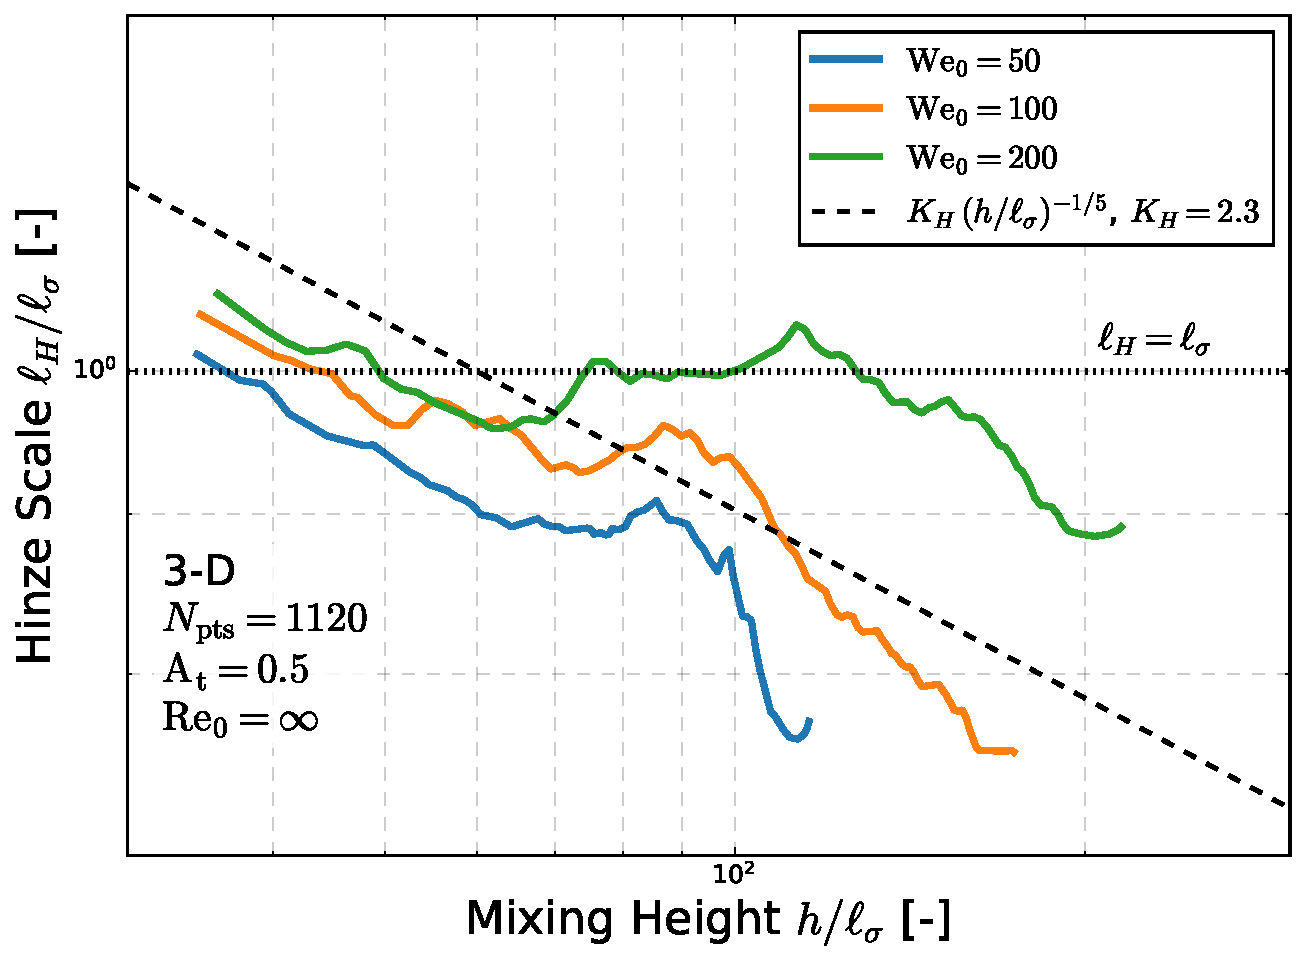
\includegraphics[width=0.6\textwidth]{figures/fig_hinze_ratio.pdf}
\caption{Hinze scale, evaluated with the dissipation rate of the simulations \cite{Walker2026,Walker2027_2}, relative to the capillary length against $h/\ls$ after the transition, with the scaling $K_H (\ls/h)^{1/5}$ of \eqref{eq:hinze_scaling} fitted with $K_H = 2.3$ (dashed). The dotted line marks $\ell_H = \ls$; below it the inner cutoff of Section~\ref{sec:scaling:closure} is $\ell_H$.}
\label{fig:hinze}
\end{figure}

\subsection{Consequences of self-similarity}\label{sec:rc:consequences}
The quantities $\sigma/\bar\rho$ and $\At g$ define the length $\ls$ but no dimensionless group. A second length is needed, and under complete self-similarity the only one available is $h$, which grows with time; the initial wavelength $\lambda_0$ is forgotten. If a self-similar state exists with $h$ as its only outer length, then $d_\sigma \rightarrowtriangle 0$ and $\alpha \rightarrowtriangle \alpha_\infty$ given by \eqref{eq:C0}, with no explicit dependence on $\sigma$. Complete self-similarity therefore excludes a persistent power law $\alpha \propto \We^{-m}$.

Two further lines of analysis are possible. First, the capillary group decays but has not yet vanished; this is incomplete similarity in the sense of Barenblatt \cite{Barenblatt1996}, and Section~\ref{sec:rc:ode} derives the resulting correction. Second, the profile constants may be inherited from the transition. RC04 note that self-similarity holds $\avg{c' c'}_\mathrm{o}$ at its value at the start of the turbulent growth phase (their \S4), and the same applies to every profile constant in \eqref{eq:C0}. During the transition, $h \sim \lambda_0$, and the capillary ratio $\ls/\lambda_0 = (2 \At \We)^{-1/2}$ from \eqref{eq:ls_We} is not small, so $\chi_0$ and $\hat D$ may depend on $\We$. The form of that dependence requires a closure, as RC04 state for $C_\mathrm{o}$.

\subsection{First-order capillary correction}\label{sec:rc:ode}
Starting from \eqref{eq:alpha_RC}, the capillary group is not constant: by \eqref{eq:dsigma} it decays as a power of $h$,
\begin{equation}\label{eq:dsigma_power}
d_\sigma = \hat d_\sigma \Big(\frac{\ls}{h}\Big)^{\nu} \, , \qquad \hat d_\sigma \sim \frac{1}{2 \alpha} \, , \qquad \nu = 2 \;,
\end{equation}
whereas $\avg{c' c'}_0$, $\chi_0$ and $\hat D$ take their self-similar values. For $h \gg \ls$, $d_\sigma \ll \hat D$ and the denominator of \eqref{eq:alpha_RC} may be expanded, $(\hat D + d_\sigma)^{-1} = \hat D^{-1}[1 - d_\sigma/\hat D + \mathcal{O}(d_\sigma^2)]$. With \eqref{eq:C0}, this gives
\begin{equation}\label{eq:cap_ode}
\hd^2 = \At g \, C_\mathrm{o} \, h \, \Big[1 - a_\sigma \Big(\frac{\ls}{h}\Big)^{\nu}\Big] \, , \qquad a_\sigma = \frac{\hat d_\sigma}{\hat D} > 0 \;,
\end{equation}
which is the modified growth equation of Section~\ref{sec:modified} with $\nu = 2$. The sign of $a_\sigma$ follows from the restoring character of the capillary force: on the tip of a falling spike, where $c' > 0$, the force points upward; on the cap of a rising bubble, where $c' < 0$, it points downward; in both cases, $c' f_z > 0$, so $d_\sigma > 0$.

Integrating \eqref{eq:cap_ode} for $h \gg \ls$ (Appendix~\ref{app:integration}) gives, for the two diagnostics \eqref{eq:alpha_defs},
\begin{align}
\alpha(t) & = \alpha_\infty \Big[1 - a_\sigma \Big(\frac{\ls}{h}\Big)^{\nu}\Big] \;, \label{eq:alpha_t_corr} \\
\alpha_{\rm eff}(t) & = \alpha_\infty \Big[1 - a_\sigma \frac{1 - \nu}{1 - 2 \nu} \Big(\frac{\ls}{h}\Big)^{\nu}
- \frac{c_v}{\sqrt h} + \dots\Big] \;, \label{eq:alpha_eff_corr}
\end{align}
where $c_v$ is set by the virtual origin. In $\alpha_{\rm eff}$, the virtual-origin term decays as $h^{-1/2}$ and dominates any correction with $\nu > 1/2$; \eqref{eq:alpha_t_corr} does not contain it. With \eqref{eq:ls_We} and \eqref{eq:ls_Wet}, \eqref{eq:alpha_t_corr} reads
\begin{equation}\label{eq:alpha_We_corr}
\alpha(t) = \alpha_\infty \Big[1 - a_\sigma \,(2 \At \We)^{-\nu/2} \Big(\frac{\lambda_0}{h}\Big)^{\nu}\Big]
= \alpha_\infty \Big[1 - a_\sigma \Big(\frac{2 \alpha}{\mathrm{We}(t)}\Big)^{\nu/2}\Big] \;.
\end{equation}
For $a_\sigma > 0$, both diagnostics decrease as $\sigma$ increases.

\subsection{Relaxation toward the self-similar state}\label{sec:rc:relax}
Equation \eqref{eq:flux_ode} also describes how a departure from $\hd^2 \propto h$ decays when the profile constants are fixed. Writing $y = \hd^2$, so that $\ddot h = \tfrac12 \, \mathrm d y/\mathrm d h$, and setting $d_\sigma = 0$, \eqref{eq:flux_ode} becomes the linear equation
\begin{equation}\label{eq:relax_ode}
\frac{\mathrm d y}{\mathrm d h} + \beta \, \frac{y}{h} = R_f \At g(1 - \chi_0) \avg{c' c'}_0 \, , \qquad
\beta = R_f \hat D - 1 \;,
\end{equation}
with solution
\begin{equation}\label{eq:relax_sol}
\hd^2 = \At g C_\mathrm{o} h + E \, h^{-\beta} \quad \rightarrowtriangle \quad
\alpha(t) - \alpha_\infty = \frac{E}{4 \At g} \, h^{-R_f \hat D} \;,
\end{equation}
where $E$ is a constant of integration. With $\alpha_\infty \approx 0.035$, $\chi_0 \approx 1/3$ and $R_f \approx 8.0$, the values without surface tension, \eqref{eq:C0} gives $\hat D \approx 4.8$, so $R_f \hat D \approx 40$. Within the RC04 balance with fixed constants, a departure from self-similar growth decays as a high power of $h$. A correction that decays only as $h^{-1}$, as in \eqref{eq:capvel}, therefore cannot be a transient of \eqref{eq:flux_ode} with fixed constants. It requires either a slow evolution of the constants $\chi_0$ and $\hat D$, or an additional term in the balance that scales as $\ls/h$.

%======================================================================
\section{A modified growth equation}\label{sec:modified}

\subsection{Statement}\label{sec:modified:statement}
The effect of surface tension on the late-time growth is written as a modification of the RC04 equation,
\begin{equation}\label{eq:mod_ode}
\hd^2 = \At g C_\mathrm{o} h \Big[1 - a \Big(\frac{\ls}{h}\Big)^{\nu}\Big] \, , \qquad C_\mathrm{o} = 4 \alpha_\infty \;,
\end{equation}
where $a$ is a constant and $\ls$ is the linear capillary cutoff \eqref{eq:dispersion}. Equation \eqref{eq:mod_ode} has the form of \eqref{eq:cap_ode} with the exponent $\nu$ left open. The exponent is related to the fractal dimension $D_s$ of the interface (Section~\ref{sec:modified:exponent}) through
\begin{equation}\label{eq:mod_nu}
\nu = \frac{6 q - 2}{5} = \frac{3 p - 5}{5} = \frac{7 - 3 D_s}{5} \;,
\end{equation}
which gives $\nu = 1/5$ for a smooth interface. For $\nu = 1/5$, the effective growth parameter follows as in RC04,
\begin{equation}\label{eq:mod_aeff}
\alpha_{\rm eff}(h) = \frac{C_\mathrm{o}}{4} \Big[1 - \frac{4 a}{3} \Big(\frac{\ls}{h}\Big)^{1/5}\Big] \;.
\end{equation}

\subsection{The exponent relations}\label{sec:modified:exponent}
The three forms of \eqref{eq:mod_nu} follow from the properties of a two-phase indicator field. For such a field, the second-order structure function $\mathcal{S}_2(r) = \avg{[c(\mathbf x + \mathbf r) - c(\mathbf x)]^2}$ is proportional to the probability that a segment of length $r$ crosses the interface. That probability scales with the surface density measured at resolution $r$, $\Sigma(r) \propto h^{-1}(h/r)^{D_s - 2}$, so $\mathcal{S}_2(r) \propto r^{3 - D_s}$ \cite{Sreenivasan1991}. Defining $q$ by $\mathcal{S}_2 \propto r^{2 q}$ and $p$ by the spectrum $E_c(k) \propto k^{-p}$, with $p = 2 q + 1$,
\begin{equation}\label{eq:pq_Ds}
D_s = 3 - 2 q = 4 - p \;.
\end{equation}
These relations make the three expressions in \eqref{eq:mod_nu} equal. A smooth interface, $D_s = 2$, has $q = 1/2$ and $p = 2$ (the spectrum of Porod \cite{Porod1951}), and gives $\nu = 1/5$. An indicator with the Obukhov--Corrsin spectrum $p = 5/3$ \cite{Obukhov1949,Corrsin1951} has $D_s = 7/3$.

The value $(6 q - 2)/5$ is obtained by estimating the capillary term at the Hinze scale: the ratio of capillary to buoyancy pressure at $\ell_H$, weighted by the relative amplitude of the indicator fluctuation at that scale,
\begin{equation}\label{eq:hinze_estimate}
\frac{\text{capillary}}{\text{buoyancy}} \sim \frac{\sigma/\ell_H}{\Delta \rho \, g \, \ell_H}
\Big(\frac{\ell_H}{h}\Big)^{q} = \Big(\frac{\ls}{\ell_H}\Big)^2 \Big(\frac{\ell_H}{h}\Big)^{q} \;.
\end{equation}
Substituting \eqref{eq:hinze_scaling} and omitting the factors of $K_H$,
\begin{equation}\label{eq:hinze_nu}
\Big(\frac{\ls}{h}\Big)^{-2/5} \Big(\frac{\ls}{h}\Big)^{6 q/5} = \Big(\frac{\ls}{h}\Big)^{(6 q - 2)/5} \;,
\end{equation}
which is \eqref{eq:mod_nu}.

\subsection{The effective growth parameter}\label{sec:modified:aeff}
Equation \eqref{eq:mod_aeff} is \eqref{eq:alpha_eff_corr} with $\nu = 1/5$, for which $(1 - \nu)/(1 - 2 \nu) = 4/3$, with the virtual-origin term omitted. The factor $4/3$ appears only in $\alpha_{\rm eff}$, which divides $\hd$ by the elapsed time and so retains the larger correction from earlier times; for $\alpha(t)$, the measure used in the simulations, the coefficient is $a$ \eqref{eq:alpha_t_corr}.

\subsection{Interpretation}\label{sec:modified:interp}
Equation \eqref{eq:mod_ode} offers a single description of the Weber-number dependence of $\alpha$ across all cases. Decreasing $\We$ increases $\ls \sim \sigma^{1/2}$ through \eqref{eq:ls_We}. In the simulations, this increases the growth rate and delays self-similarity, and the curves eventually converge (Section~\ref{sec:sims}). The leading-order term of \eqref{eq:mod_ode} is the RC04 equation and gives the standard $\alpha$. The additional term shifts $\alpha$ relative to the $\We = \infty$ case, and the shift decreases as $h$ grows, so all cases approach $\alpha_\infty$ as $h/\ls \rightarrowtriangle \infty$, consistent with Section~\ref{sec:rc:consequences}. A shift that decreases with $h$ is what is required for the simulations at different Weber numbers to collapse on a single curve. Compared at equal mixing width, they do correspond to a single function of $\ls/h$ (Section~\ref{sec:sims:width}).

Three points constrain the form of the correction. First, the sign: with $a > 0$, $\alpha(t)$ \eqref{eq:alpha_t_corr} decreases as $\ls$ increases, and so does $\alpha_{\rm eff}$ \eqref{eq:alpha_eff_corr} for $\nu < 1/2$ or $\nu > 1$, where $(1 - \nu)/(1 - 2 \nu) > 0$; the observed increase of $\alpha$ therefore requires $a < 0$. A restoring capillary force gives $a > 0$ (Section~\ref{sec:rc:ode}), so a negative $a$ must come from an indirect effect of surface tension on the flow structure. Second, the exponent: the fit in Section~\ref{sec:sims:width} has $\nu \approx 1$, whereas \eqref{eq:mod_nu} gives $\nu \le 1/5$ for $D_s \ge 2$. Moreover, $\nu > 0$ in \eqref{eq:mod_nu} requires $D_s < 7/3$; at $D_s = 7/3$, the term renormalizes $C_\mathrm{o}$, and for the values $D_s \approx 2.6$--$2.7$ reported for scalar iso-surfaces in turbulence \cite{Sreenivasan1991}, $\nu < 0$ and the correction would grow with $h$. Third, the magnitude: with $\nu = 1$ the fit gives $\alpha - \alpha_\infty \approx 8.9 \, \ls/h$, which in the normalization of \eqref{eq:mod_ode} is $a \approx -8.9/\alpha_\infty \approx -250$. The correction is of order unity relative to $\alpha_\infty$ over the simulated range, and $|a|$ is much larger than unity.

%======================================================================
\section{Mass-flux formulation}\label{sec:cook}

\subsection{Growth and mid-plane mass flux}\label{sec:cook:flux}
For incompressible phases $\avg\rho = \rho_\ell + \Delta \rho \bar V$, and mean continuity gives
\begin{equation}\label{eq:continuity}
\Delta \rho \, \pd{\bar V}{t} = -\pd{}{z} \avg{\rho w} \;.
\end{equation}
Differentiating \eqref{eq:h} and integrating by parts, with $\avg{\rho w} \rightarrowtriangle 0$ as $| z | \rightarrowtriangle \infty$,
\begin{equation}\label{eq:hdot_flux}
\hd = -\frac{12}{\Delta \rho} \int_{-\infty}^{\infty} \avg{\rho w} \, \pd{\bar V}{z} \, \mathrm d z \;.
\end{equation}
For immiscible incompressible phases, $\avg w = 0$, so $\avg{\rho w} = \avg{\rho' w'}$. CCM04 obtain the corresponding result for their entrainment length $h_C$ (their eqs.~3.5 and 7.3), and approximate it as $\hd_C \approx -4 \avg{\rho w}_0/\Delta \rho$ (their eq.~7.4).

Define the shape factor
\begin{equation}\label{eq:Rf}
R_f \equiv \frac{\Delta \rho \, \hd}{| \avg{\rho' w'}_0 |} \;,
\end{equation}
twice the ``scaling ratio'' reported in Refs.~\cite{Walker2026,Walker2027_1}, which uses the half-width $h/2$. For a self-similar profile, $\avg{\rho w}_0 = -\Delta \rho \,(\mathrm d/\mathrm d t) \int_{-\infty}^0 \bar V \, \mathrm d z$, so $R_f$ depends only on the shape of $\bar V$:
\begin{equation}\label{eq:Rf_values}
R_f = \frac{h}{\int_{-\infty}^0 \bar V \, \mathrm d z} = \frac{4 h}{h_C} =
\begin{cases} 8 & \text{linear profile} \;, \\ 6 \sqrt2 \approx 8.49 & \text{error-function profile} \;, \\
6/\ln 2 \approx 8.66 & \tanh \  \text{profile} \;. \end{cases}
\end{equation}
The value $R_f = 4$ corresponds to the entrainment length of CCM04; for the full width \eqref{eq:h}, the self-similar value is $8.0$--$8.7$. Without surface tension, $R_f$ rises into the self-similar range at late times, with a mean of $8.0$ over $8 \le t/\tau_0 \le 9.4$, the value for a linear profile; with surface tension it settles at $9.7$--$10.7$, above that range, and in the miscible case it is still increasing (Figure~\ref{fig:Rf}, Table~\ref{tab:decomp}).

\begin{figure}[h!]
\centering
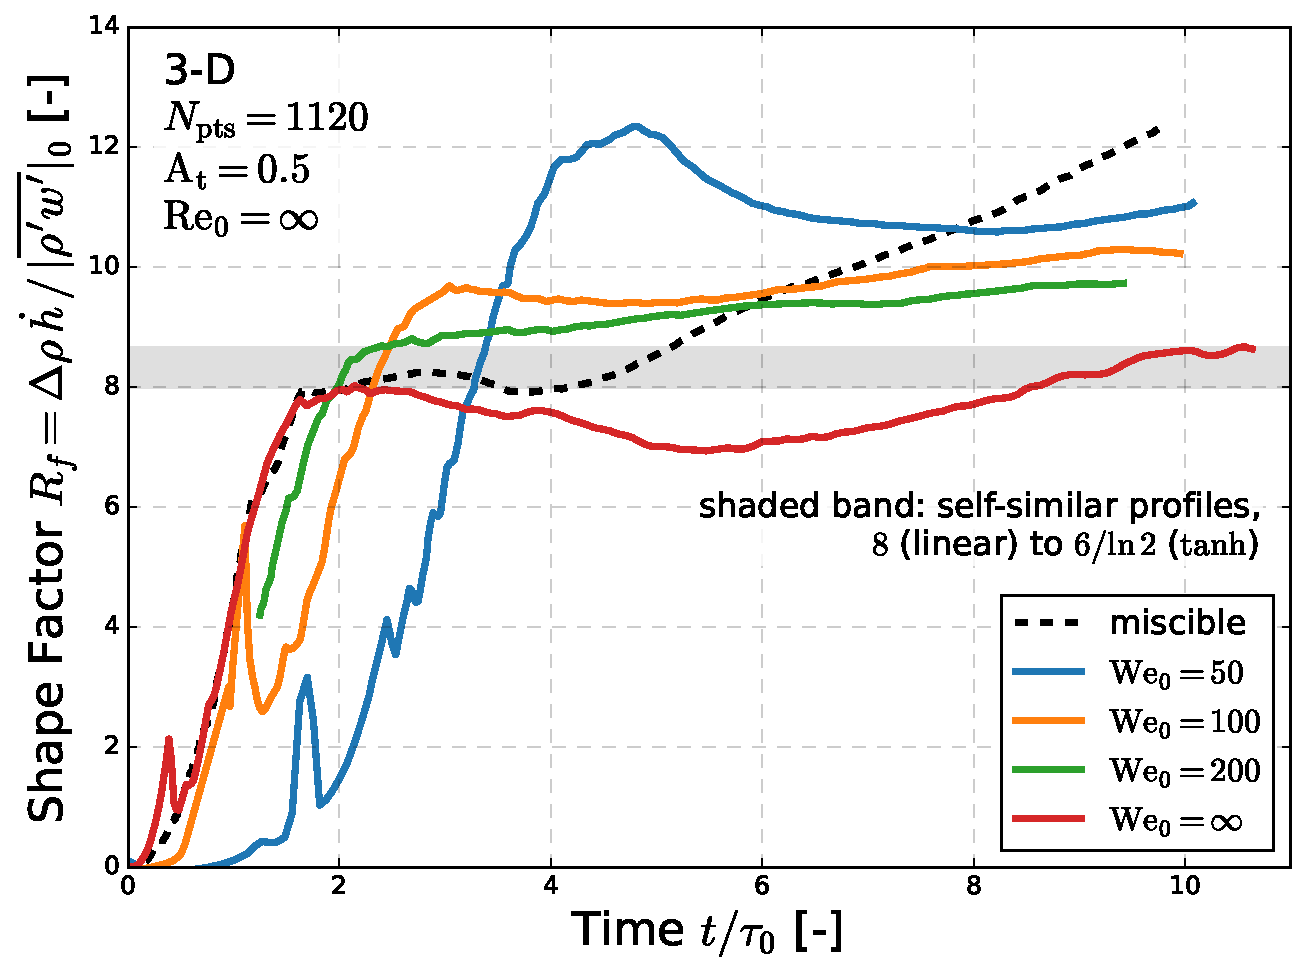
\includegraphics[width=0.6\textwidth]{figures/fig_Rf_time.pdf}
\caption{Mass-flux shape factor $R_f = \Delta \rho \, \hd/| \avg{\rho' w'}_0 |$ for the full width \eqref{eq:h}, twice the scaling ratio of Refs.~\cite{Walker2026,Walker2027_1}. The gray band marks the self-similar values \eqref{eq:Rf_values}.}
\label{fig:Rf}
\end{figure}

\subsection{Decomposition of the growth parameter}\label{sec:cook:decomp}
Following CCM04 (their eq.~7.5), write $\avg{\rho' w'}_0 = -C_r \rho_{\rm rms} w_{\rm rms}$, with $\rho_{\rm rms} = \Delta \rho \,[\bar V_0(1 - \bar V_0)(1 - \theta_0)]^{1/2}$, where $\theta_0$ is the mid-plane mixedness, and define $\mathrm{Fr}_0^2 = w_{\rm rms}^2/(\At g h)$. With $\bar V_0 = 1/2$, \eqref{eq:alpha_defs} and \eqref{eq:Rf} give
\begin{equation}\label{eq:decomp}
\alpha = \frac{R_f^2}{16} \, C_r^2 \,(1 - \theta_0) \, \mathrm{Fr}_0^2 \;.
\end{equation}
The effective Atwood number of CCM04 (their eq.~3.14) is $\mathrm{A}_\mathrm{eff} = \At(1 - \theta_0)^{1/2}$ in this notation. Their closure $w_{\rm rms} = C_w(\mathrm{A}_\mathrm{eff} g h)^{1/2}$ (eq.~7.8) gives $\mathrm{Fr}_0^2 = C_w^2(1 - \theta_0)^{1/2}$ and hence
\begin{equation}\label{eq:cook_closure}
\alpha = \frac{R_f^2}{16} \, C_r^2 C_w^2 \,(1 - \theta_0)^{3/2} = \frac{R_f^2}{16} \, C_r^2 C_w^2 \Big(\frac{\mathrm{A}_\mathrm{eff}}{\At}\Big)^3 \;,
\end{equation}
which reduces to CCM04 eq.~7.12 for $R_f = 4$.

\subsection{Application to the simulation values}\label{sec:cook:table}
Table~\ref{tab:decomp} applies \eqref{eq:decomp} to the simulations of Refs.~\cite{Walker2026,Walker2027_1,Walker2027_2}, averaged over $8 \le t/\tau_0 \le 9.4$, with $\theta_0$ obtained from the mid-plane density fluctuation, $1 - \theta_0 = (2 \rho_{\rm rms}/\Delta \rho)^2$.
\begin{table}[h!]
\centering
\caption{Decomposition \eqref{eq:decomp} of the growth parameter, averaged over $8 \le t/\tau_0 \le 9.4$, with $R_f$ for the full width \eqref{eq:h} and $\theta_0$ from the mid-plane density fluctuation (3-D, $N_\mathrm{pts} = 1120$, $\At = 0.5$, $\mathrm{Re}_0 = \infty$).}
\label{tab:decomp}
\begin{tabular}{lccccc}
\toprule
case & $\alpha$ & $R_f$ & $\theta_0$ & $C_r^2 \mathrm{Fr}_0^2 = 16 \alpha/[R_f^2(1 - \theta_0)]$ & $C_r \mathrm{Fr}_0$\\
\midrule
$\We = 50$ & 0.132 & 10.7 & 0.10 & 0.0206 & 0.144\\
$\We = 100$ & 0.105 & 10.2 & 0.13 & 0.0189 & 0.138\\
$\We = 200$ & 0.078 & 9.7 & 0.19 & 0.0166 & 0.129\\
$\We = \infty$ & 0.034 & 8.0 & 0.40 & 0.0141 & 0.119\\
miscible & 0.023 & 11.4 & 0.86 & 0.0198 & 0.141\\
\bottomrule
\end{tabular}
\end{table}

Between $\We = 50$ and $\We = \infty$, the factor $3.84$ in $\alpha$ splits as $1.76$ from $R_f^2$, $1.49$ from $1 - \theta_0$ and $1.46$ from $C_r^2 \mathrm{Fr}_0^2$. Between $\We = \infty$ and the miscible case, the factor $1.51$ splits as $0.50 \times 4.25 \times 0.71$. The closure \eqref{eq:cook_closure} would predict $4.25^{3/2} \approx 8.8$ for the latter, and a closure linear in $1 - \theta_0$ with the other constants fixed would predict $4.3$. The purity factor alone therefore overpredicts the difference between miscible and immiscible growth. The immiscible case without surface tension has a higher purity than the miscible case but the lowest $R_f$ and $C_r \mathrm{Fr}_0$ of all five cases; surface tension raises $R_f^2$, the purity and $C_r^2 \mathrm{Fr}_0^2$ by comparable factors. Within \eqref{eq:decomp}, the $\We$ dependence is shared among the three factors, and $R_f^2$ is the largest.

\subsection{Energy budget}\label{sec:cook:energy}
Let $P_{\rm rel} = c_P \, \Delta \rho \, g h^2$ be the released potential energy per unit horizontal area ($c_P = 1/24$ for a linear profile), $K_E = c_K \bar\rho \, \hd^2 h$ the kinetic energy per unit area, $E_\varepsilon$ the dissipated energy and $S(t)$ the interface area per unit horizontal area. Conservation of energy, $P_{\rm rel} = K_E + E_\varepsilon + \sigma(S - 1)$, together with $\hd^2 = 4 \alpha \At g h$, gives
\begin{equation}\label{eq:energy}
\alpha = \frac{c_P}{2 c_K} \, \frac{K_E}{P_{\rm rel}} = \frac{c_P}{2 c_K} \big(1 - \Phi_\varepsilon - \Phi_\sigma\big) \, , \qquad
\Phi_\varepsilon = \frac{E_\varepsilon}{P_{\rm rel}} \, , \quad \Phi_\sigma = \frac{\sigma(S - 1)}{P_{\rm rel}} \ge 0 \;.
\end{equation}
The surface energy term lowers $\alpha$. An increase of $\alpha$ with $\sigma$ must therefore come from a smaller dissipated fraction $\Phi_\varepsilon$ or from a change in the shape ratio $c_P/c_K$. At $\mathrm{Re}_0 = \infty$, $\Phi_\varepsilon$ is the numerical dissipation of the scheme \cite{Cook2007,Brill2025}.

%======================================================================
\section{Scaling of \texorpdfstring{$\alpha$}{alpha} with \texorpdfstring{$\We$}{We0}}\label{sec:scaling}

\subsection{Complete self-similarity}\label{sec:scaling:rc}
Under the RC04 assumption that energy-containing quantities scale with $h$, the capillary group decays as $(\ls/h)^2$ (Section~\ref{sec:rc:capillary}), and \eqref{eq:alpha_We_corr} with $\nu = 2$ gives
\begin{equation}\label{eq:scaling_rc}
\alpha(t) = \alpha_\infty \Big[1 - \frac{a_\sigma}{2 \At \We} \Big(\frac{\lambda_0}{h}\Big)^2\Big]
= \alpha_\infty \Big[1 - \frac{2 \alpha \, a_\sigma}{\mathrm{We}(t)}\Big] \;.
\end{equation}
The correction is proportional to $\We^{-1}$ (so linear in $\sigma$); it reduces $\alpha$ and decays as $h^{-2}$, and $\alpha_\infty = C_\mathrm{o}/4$ carries no $\We$ dependence. The only other choice consistent with RC04 is a constant capillary group, $\Gamma_0 \propto \ls^{-2}$ for the capillary moment $\avg{c' f_z} = (\sigma/\bar\rho) \Gamma$. That shifts $C_\mathrm{o}$ by a pure number independent of $\lambda_0$ and again gives no $\We$ scaling. Since $\We^{-1/2} = \ls/\lambda_0$ at $\At = 0.5$, a $\We^{-1/2}$ scaling requires the capillary length to enter linearly ($\nu = 1$) at the energy-containing level. Self-similarity does not supply this; it requires a closure for $C_\mathrm{o}$, which RC04 leave open.

\subsection{A spectral closure beyond Ristorcelli \& Clark}\label{sec:scaling:closure}
The closure in this subsection is not part of RC04. It uses the interface fractal dimension of Section~\ref{sec:modified:exponent}.

\paragraph{Terms through which $\sigma$ can act.} By \eqref{eq:cc0}, $\avg{c' c'}_0 = 1$ for immiscible fluids, so $\sigma$ can act on \eqref{eq:alpha_RC} only through the terms in Table~\ref{tab:terms}. Here $D_s$ is the fractal dimension of the interface, $\ell_{\rm in}$ its inner cutoff, and the interface is assumed fractal between $\ell_H$ and $h$ when estimating the surface energy.
\begin{table}[h!]
\centering
\caption{Terms through which surface tension can modify \eqref{eq:alpha_RC}, with their magnitude relative to buoyancy.}
\label{tab:terms}
\begin{tabular}{lll}
\toprule
term & relative magnitude & effect on $\alpha$\\
\midrule
capillary force in the flux budget, $d_\sigma$ \eqref{eq:dsigma} & $(\ls/h)^2$ & decrease\\
surface energy in the energy budget, $\Phi_\sigma$ \eqref{eq:energy} & $(\ls/h)^{(22 - 6 D_s)/5}$ & decrease\\
inner cutoff of the indicator spectrum & $(\ell_{\rm in}/h)^{3 - D_s}$ & increase\\
\bottomrule
\end{tabular}
\end{table}
For $2 \le D_s < 3$ the third term has the smallest exponent and is therefore the leading correction as $h/\ls \rightarrowtriangle \infty$. It is also the only one that increases $\alpha$.

\paragraph{Closure hypothesis.} Only the indicator variance at the energy-containing scales drives the energy-containing flux. Flux produced at small scales is destroyed locally, as in the $k^{-7/3}$ range of the scalar-flux co-spectrum \cite{Lumley1967}, and the mid-plane flux $F = 2 \hd/R_f$ is carried by the large scales. Accordingly, $\avg{c' c'}_0$ in \eqref{eq:alpha_RC} is replaced by $F_L \avg{c' c'}_0$, where $F_L$ is the fraction of the variance in the energy-containing range.

\paragraph{Spectral fraction.} For an interface of dimension $D_s$ between $\ell_{\rm in}$ and $h$, $E_c(k) \propto k^{D_s - 4}$ by \eqref{eq:pq_Ds}. Integrating over $1/h \le k \le 1/\ell_{\rm in}$,
\begin{equation}\label{eq:FL}
F_L = \frac{\int_{1/h}^{2/h} E_c \, \mathrm d k}{\int_{1/h}^{1/\ell_{\rm in}} E_c \, \mathrm d k}
= \frac{1 - 2^{D_s - 3}}{1 - (\ell_{\rm in}/h)^{3 - D_s}} \;,
\end{equation}
and therefore
\begin{equation}\label{eq:alpha_closure}
\alpha(h) = \frac{\alpha_\infty}{1 - (\ell_{\rm in}/h)^{3 - D_s}} \approx
\alpha_\infty \Big[1 + \Big(\frac{\ell_{\rm in}}{h}\Big)^{3 - D_s}\Big] \;.
\end{equation}
Without surface tension, an immiscible indicator has no inner cutoff, $\ell_{\rm in} \rightarrowtriangle 0$; surface tension sets a finite $\ell_{\rm in}$. In the simulations, surface tension interrupts the inertial cascade: turbulent kinetic energy builds up near the Hinze scale, and the density spectra change accordingly \cite{Walker2027_2}.

\paragraph{Inner cutoff.} Turbulence cannot deform the interface below $\ell_H$ \eqref{eq:hinze}, and buoyancy cannot deform it below $\ls$ \eqref{eq:dispersion}. The smaller of the two applies. By \eqref{eq:hinze_scaling}, $\ell_{\rm in} = \ls$ for $h/\ls \lesssim K_H^5$, a few hundred for $K_H = 3.3$, and $\ell_{\rm in} = \ell_H$ beyond. In the simulations, $K_H^5 \approx 60$ and $h/\ls$ reaches $100$--$215$, so $\ell_H$ is slightly smaller than $\ls$ at late times; the two cutoffs differ by less than $25\%$ (Figure~\ref{fig:hinze}), and the simulations cannot distinguish the two branches of \eqref{eq:We_scaling}, which for $D_s = 2$ give $\nu = 1$ and $\nu = 6/5$.

\paragraph{Result.} Substituting \eqref{eq:ls_We} and \eqref{eq:hinze_scaling} into \eqref{eq:alpha_closure},
\begin{equation}\label{eq:We_scaling}
\frac{\alpha - \alpha_\infty}{\alpha_\infty} \approx
\begin{cases}
(2 \At \We)^{-(3 - D_s)/2} \, \big(\lambda_0/h\big)^{3 - D_s} \, , & h/\ls \lesssim K_H^5 \;, \\[4pt]
K_H^{3 - D_s} \,(2 \At \We)^{-3(3 - D_s)/5} \, \big(\lambda_0/h\big)^{6(3 - D_s)/5} \, , & h/\ls \gtrsim K_H^5 \;.
\end{cases}
\end{equation}
For $D_s = 7/3$, this gives $\alpha - \alpha_\infty \propto \We^{-1/3}$ in the intermediate regime and $\propto \We^{-2/5}$ asymptotically. In the self-similar regime $h/\lambda_0 = \alpha_\infty(t/\tau_0)^2$, so at fixed $t/\tau_0$ the same $\We$ exponents hold, with time factors $(t/\tau_0)^{-4/3}$ and $(t/\tau_0)^{-8/5}$ respectively. A $\We^{-1/2}$ scaling requires $D_s = 2$ with $\ell_{\rm in} = \ls$, or $D_s = 13/6$ with $\ell_{\rm in} = \ell_H$. In the form \eqref{eq:mod_ode}, \eqref{eq:alpha_closure} corresponds to $a < 0$ and $\nu = 3 - D_s$ or $\nu = \tfrac65(3 - D_s)$. As $h/\ls \rightarrowtriangle \infty$, the correction vanishes, consistent with Section~\ref{sec:rc:consequences}.

\subsection{A correction linear in \texorpdfstring{$\ls/h$}{l_sigma/h}}\label{sec:scaling:linear}
The case $\nu = 1$ has three equivalent forms. It is the capillary-velocity form \eqref{eq:capvel}, $\alpha - \alpha_\infty = K \ls/h$; it is \eqref{eq:mod_ode} with $\nu = 1$ and $a = -K/\alpha_\infty$; and it is the spectral closure \eqref{eq:alpha_closure} with $D_s = 2$ and $\ell_{\rm in} = \ls$, for which $K = \alpha_\infty$. In terms of the instantaneous Weber number, by \eqref{eq:ls_Wet},
\begin{equation}\label{eq:linear_We}
\alpha(t) - \alpha_\infty = K \Big(\frac{2 \alpha}{\mathrm{We}(t)}\Big)^{1/2}
= K \,(2 \At \We)^{-1/2} \, \frac{\lambda_0}{h} \;.
\end{equation}
At fixed $h/\lambda_0$, the correction is proportional to $\We^{-1/2}$, and it decays as $h^{-1}$. By Section~\ref{sec:rc:relax}, a correction of this form is not a transient of the RC04 balance with fixed constants, which relaxes as $h^{-R_f \hat D}$ with $R_f \hat D \approx 40$.

\subsection{Comparison}\label{sec:scaling:compare}
Table~\ref{tab:compare} and Figure~\ref{fig:nu} summarize the exponents obtained above together with those inferred from the simulations in Section~\ref{sec:sims}.
\begin{table}[h!]
\centering
\caption{Dependence of $\alpha$ on $\We$ from Sections~\ref{sec:setup}--\ref{sec:scaling} and from the simulations (Section~\ref{sec:sims}). Here $\nu$ is the exponent in $(\ls/h)^{\nu}$.}
\label{tab:compare}
\begin{tabular}{llll}
\toprule
approach & $\nu$ & $\We$ dependence & effect of $\sigma$\\
\midrule
complete self-similarity, \eqref{eq:scaling_rc} & $2$ & $\alpha - \alpha_\infty \propto -\We^{-1}$ & decrease\\
Hinze-scale estimate, \eqref{eq:mod_ode}--\eqref{eq:mod_nu} & $(7 - 3 D_s)/5$ & $\alpha - \alpha_\infty \propto -\We^{-\nu/2}$ & decrease ($a > 0$)\\
spectral closure, $\ell_{\rm in} = \ls$, \eqref{eq:We_scaling} & $3 - D_s$ & $\alpha - \alpha_\infty \propto \We^{-(3 - D_s)/2}$ & increase\\
spectral closure, $\ell_{\rm in} = \ell_H$, \eqref{eq:We_scaling} & $\tfrac65(3 - D_s)$ & $\alpha - \alpha_\infty \propto \We^{-3(3 - D_s)/5}$ & increase\\
capillary velocity, \eqref{eq:capvel} & $1$ & $\alpha - \alpha_\infty \propto \We^{-1/2}$ & increase ($K > 0$)\\
simulations, fixed $t/\tau_0$ (Table~\ref{tab:fixed_time}) & --- & $\alpha \propto \We^{-0.37}$ to $\We^{-0.46}$ & increase\\
simulations, fixed $h/\lambda_0$ (Figure~\ref{fig:excess}) & $0.97$ & $\alpha - \alpha_\infty \approx 8.9 \, \ls/h$ & increase\\
\bottomrule
\end{tabular}
\end{table}

\begin{figure}[h!]
\centering
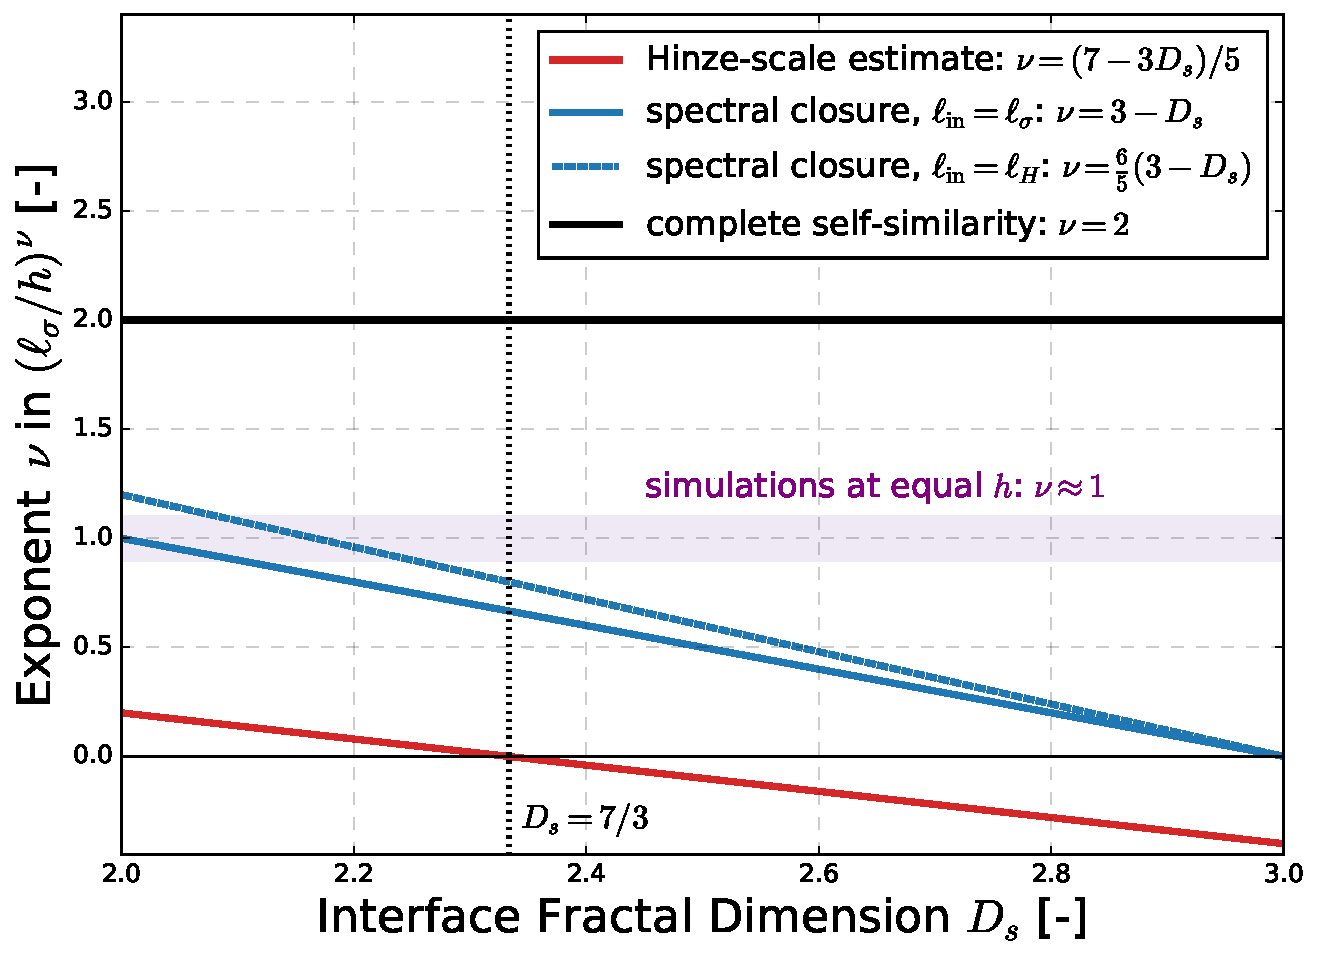
\includegraphics[width=0.6\textwidth]{figures/fig_nu_Ds.pdf}
\caption{Exponent $\nu$ of the correction $(\ls/h)^{\nu}$ as a function of the interface fractal dimension $D_s$: the Hinze-scale estimate \eqref{eq:mod_nu}, the spectral closure \eqref{eq:We_scaling} with $\ell_{\rm in} = \ls$ and $\ell_{\rm in} = \ell_H$, and complete self-similarity \eqref{eq:dsigma_power}. The shaded band marks the value $\nu \approx 1$ obtained from the simulations at equal mixing width (Figure~\ref{fig:excess}).}
\label{fig:nu}
\end{figure}

%======================================================================
\section{Simulation results}\label{sec:sims}

Figures~\ref{fig:misc} and \ref{fig:imm} reproduce the growth parameter, mixing height and growth velocity presented in Refs.~\cite{Walker2025,Walker2026}. Figures~\ref{fig:transition}--\ref{fig:capgroup} are derived from the curves of Figure~\ref{fig:imm}; the mixing height on its vertical axis satisfies $h/\lambda_0 = (\hd/\sqrt{\At g \lambda_0})^2/4 \alpha$ to within about 5\%.

\begin{figure}[h!]
\centering
\begin{subfigure}[t]{0.33\textwidth}\centering
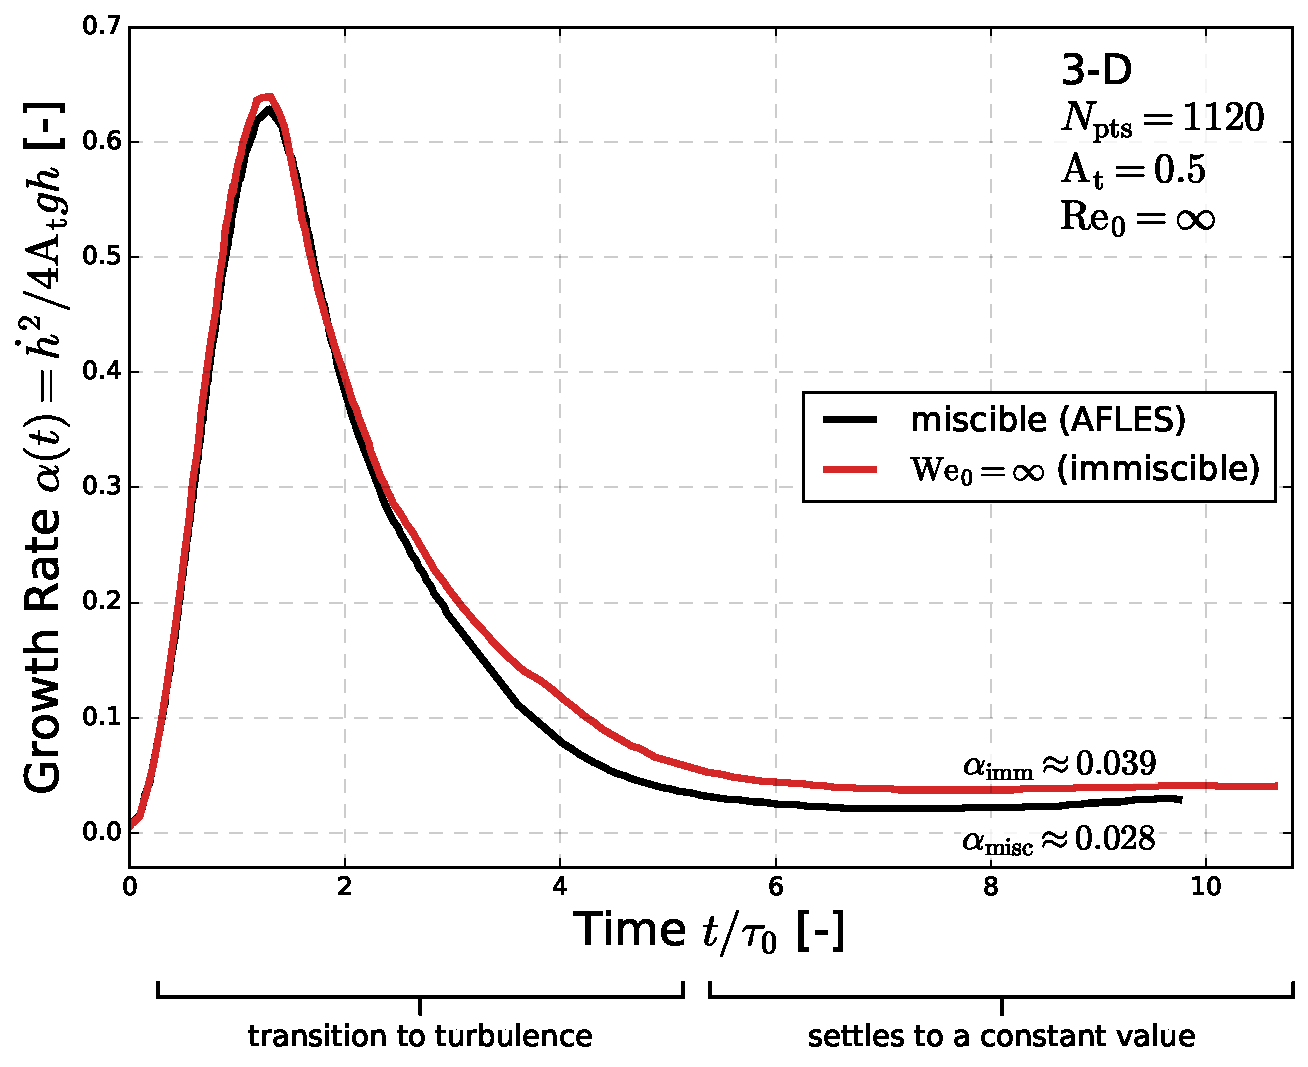
\includegraphics[width=\linewidth]{figures/simulations/alpha_time_misc_imm.pdf}\caption{}\label{fig:misc:alpha}
\end{subfigure}\hfill
\begin{subfigure}[t]{0.333\textwidth}\centering
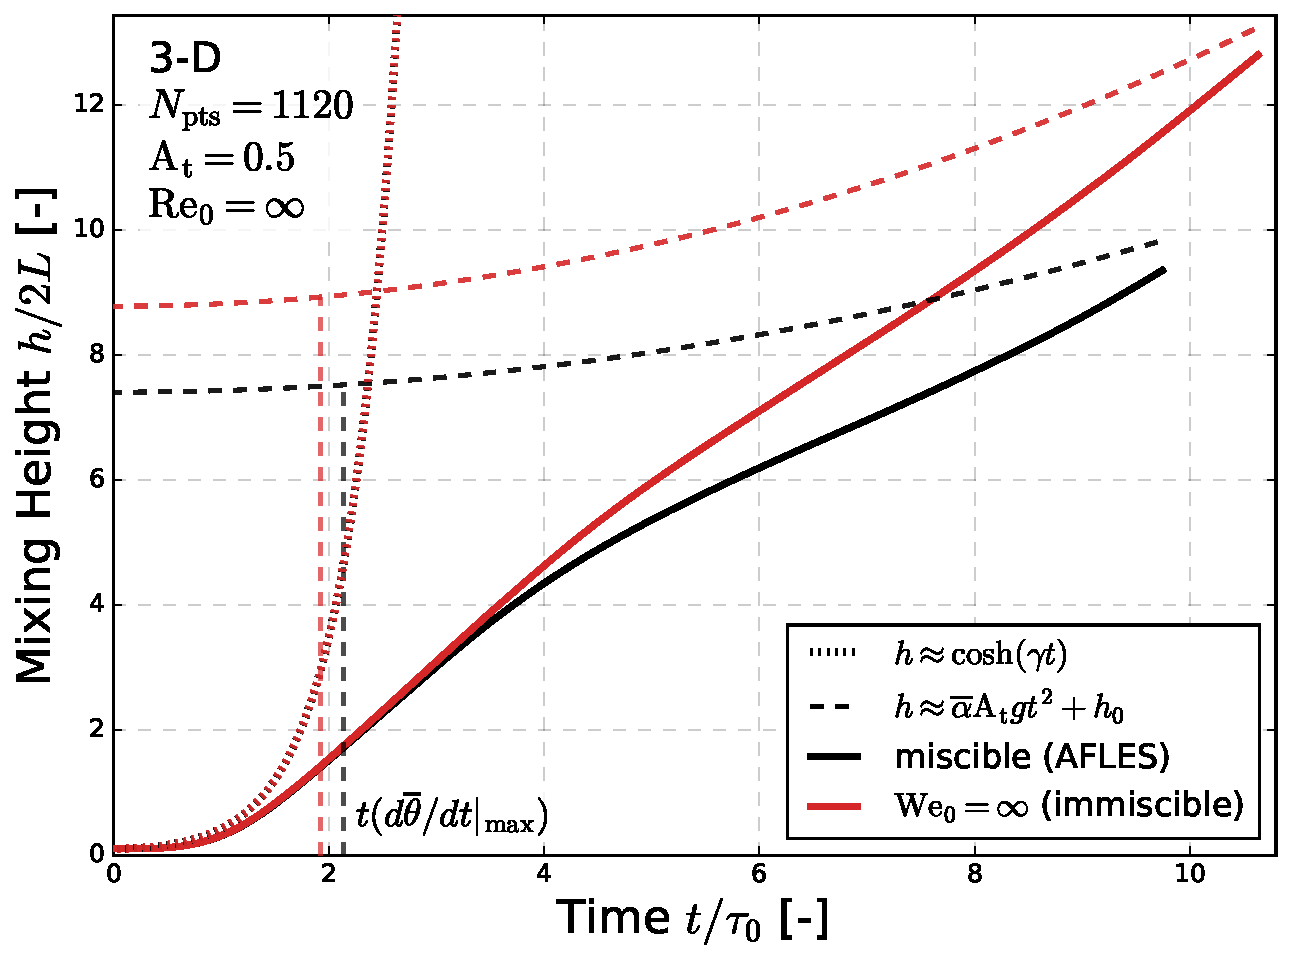
\includegraphics[width=\linewidth]{figures/simulations/alpha_time_misc_imm_height.pdf}\caption{}\label{fig:misc:h}
\end{subfigure}\hfill
\begin{subfigure}[t]{0.333\textwidth}\centering
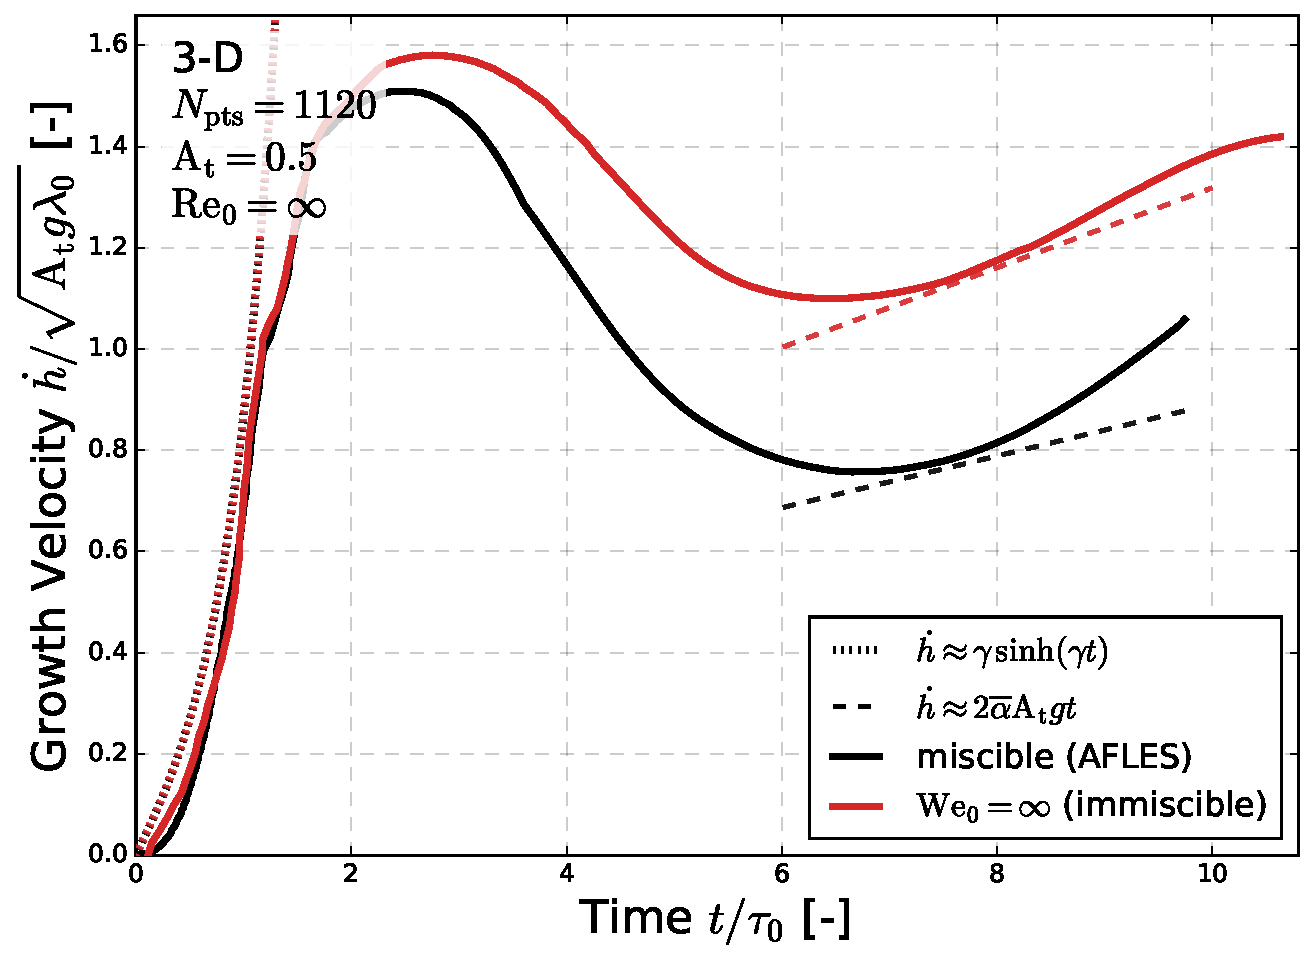
\includegraphics[width=\linewidth]{figures/simulations/alpha_time_misc_imm_velocity.pdf}\caption{}\label{fig:misc:hdot}
\end{subfigure}
\caption{Miscible (AFLES) and immiscible ($\We = \infty$) simulations, 3-D, $N_\mathrm{pts} = 1120$, $\At = 0.5$, $\mathrm{Re}_0 = \infty$ \cite{Walker2025,Walker2026}. (a) Growth parameter $\alpha(t)$ \eqref{eq:alpha_defs}. (b) Mixing height with the linear-theory solution $h \propto \cosh(\gamma t)$ (dotted) and the fit $h \approx \bar\alpha \At g t^2 + h_0$ (dashed); vertical lines mark the time of maximum $\mathrm d \bar\theta/\mathrm d t$. (c) Growth velocity $\hd/(\At g \lambda_0)^{1/2}$ with $\hd \propto \gamma \sinh(\gamma t)$ (dotted) and $\hd \approx 2 \bar\alpha \At g t$ (dashed).}
\label{fig:misc}
\end{figure}

\begin{figure}[h!]
\centering
\begin{subfigure}[t]{0.33\textwidth}\centering
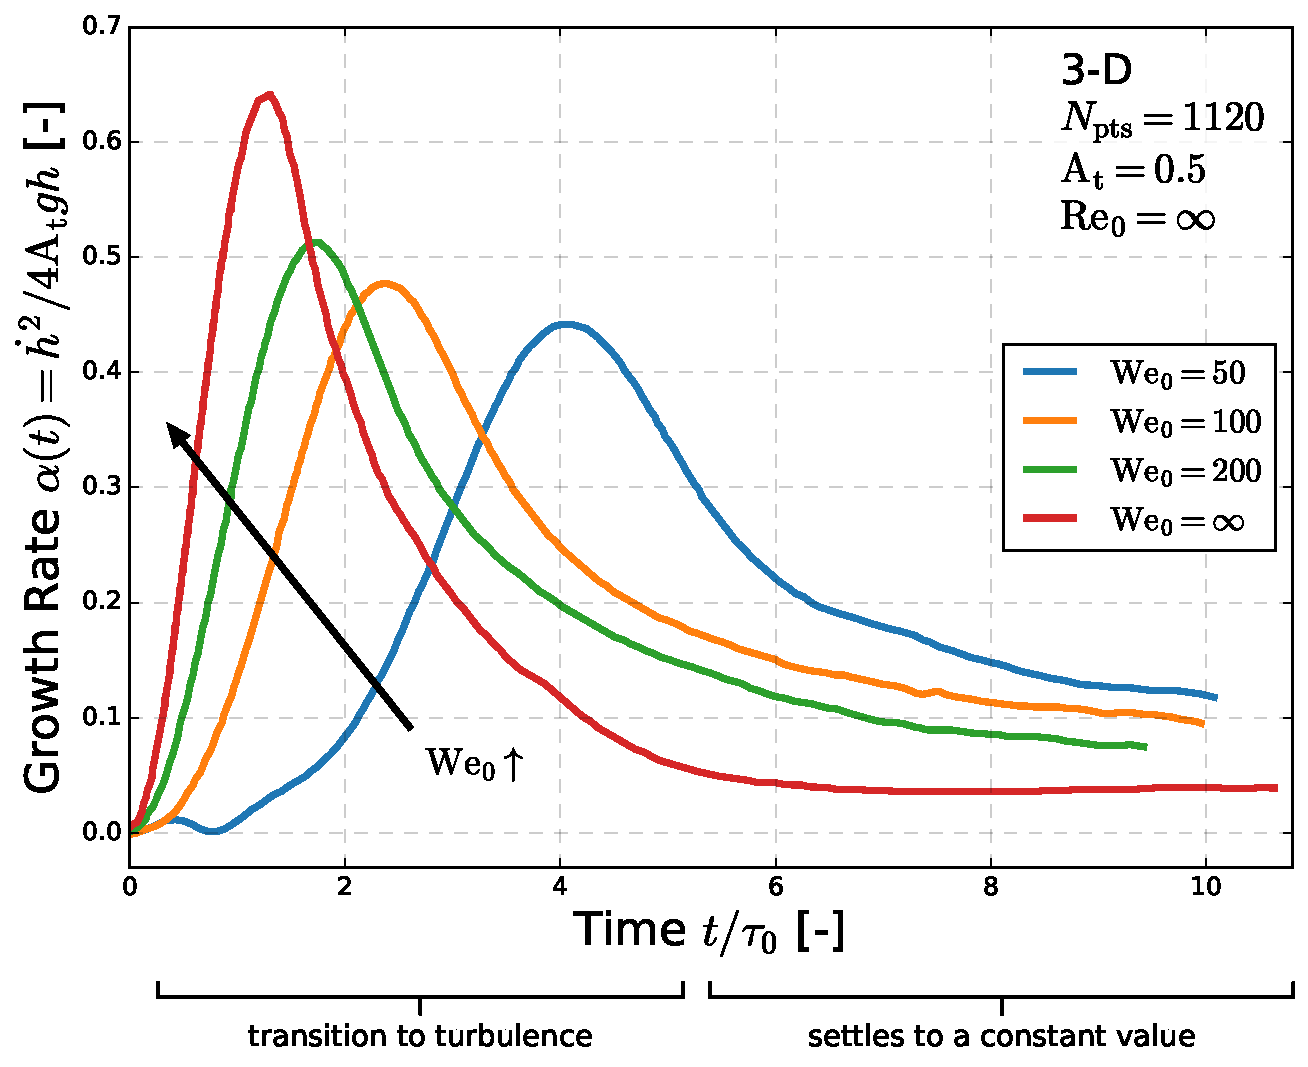
\includegraphics[width=\linewidth]{figures/simulations/immiscible_alpha_time.pdf}\caption{}\label{fig:imm:alpha}
\end{subfigure}\hfill
\begin{subfigure}[t]{0.333\textwidth}\centering
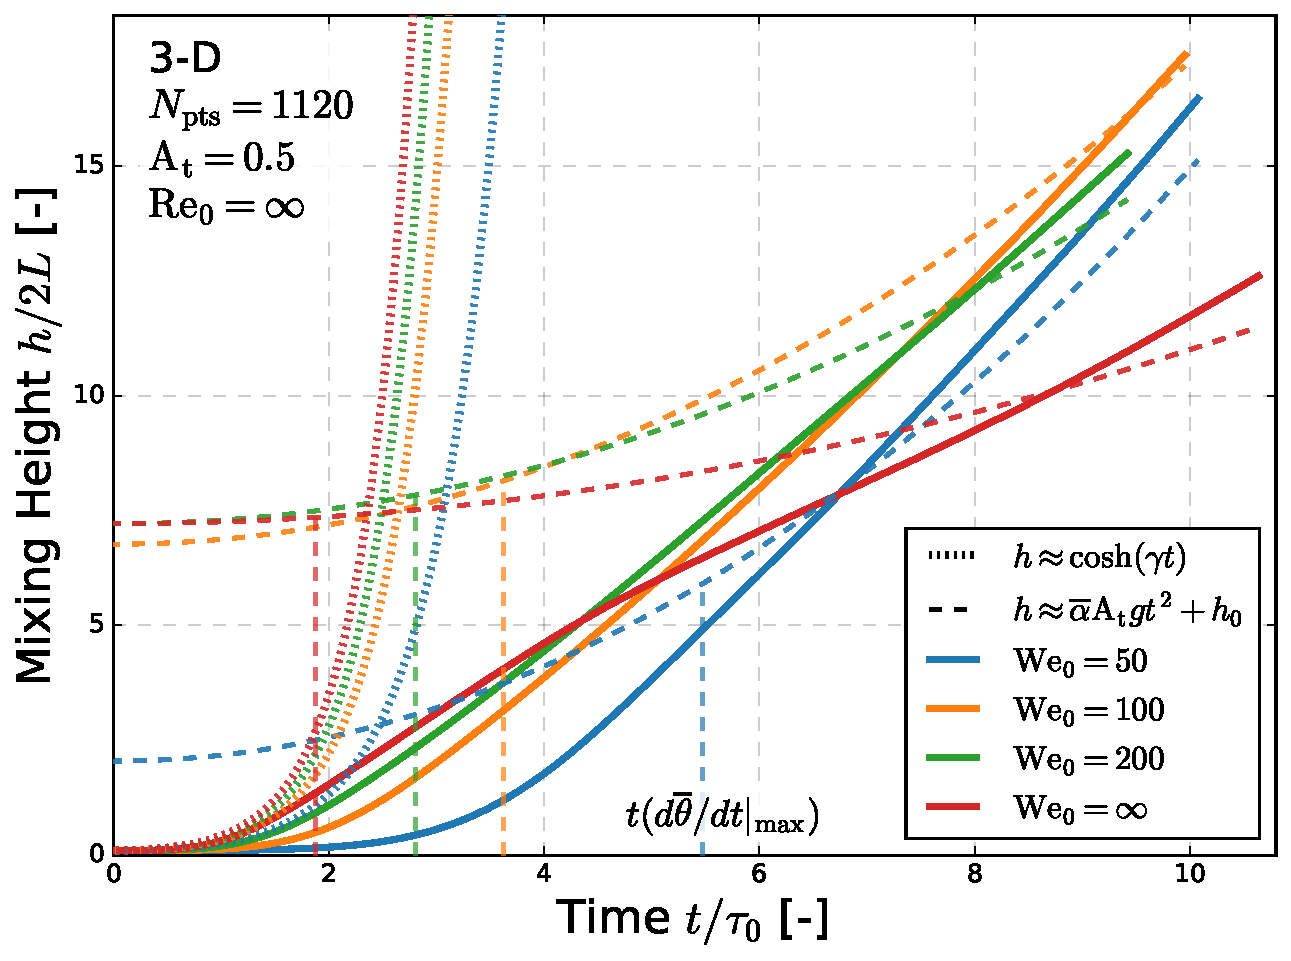
\includegraphics[width=\linewidth]{figures/simulations/immiscible_alpha_time_height.pdf}\caption{}\label{fig:imm:h}
\end{subfigure}\hfill
\begin{subfigure}[t]{0.333\textwidth}\centering
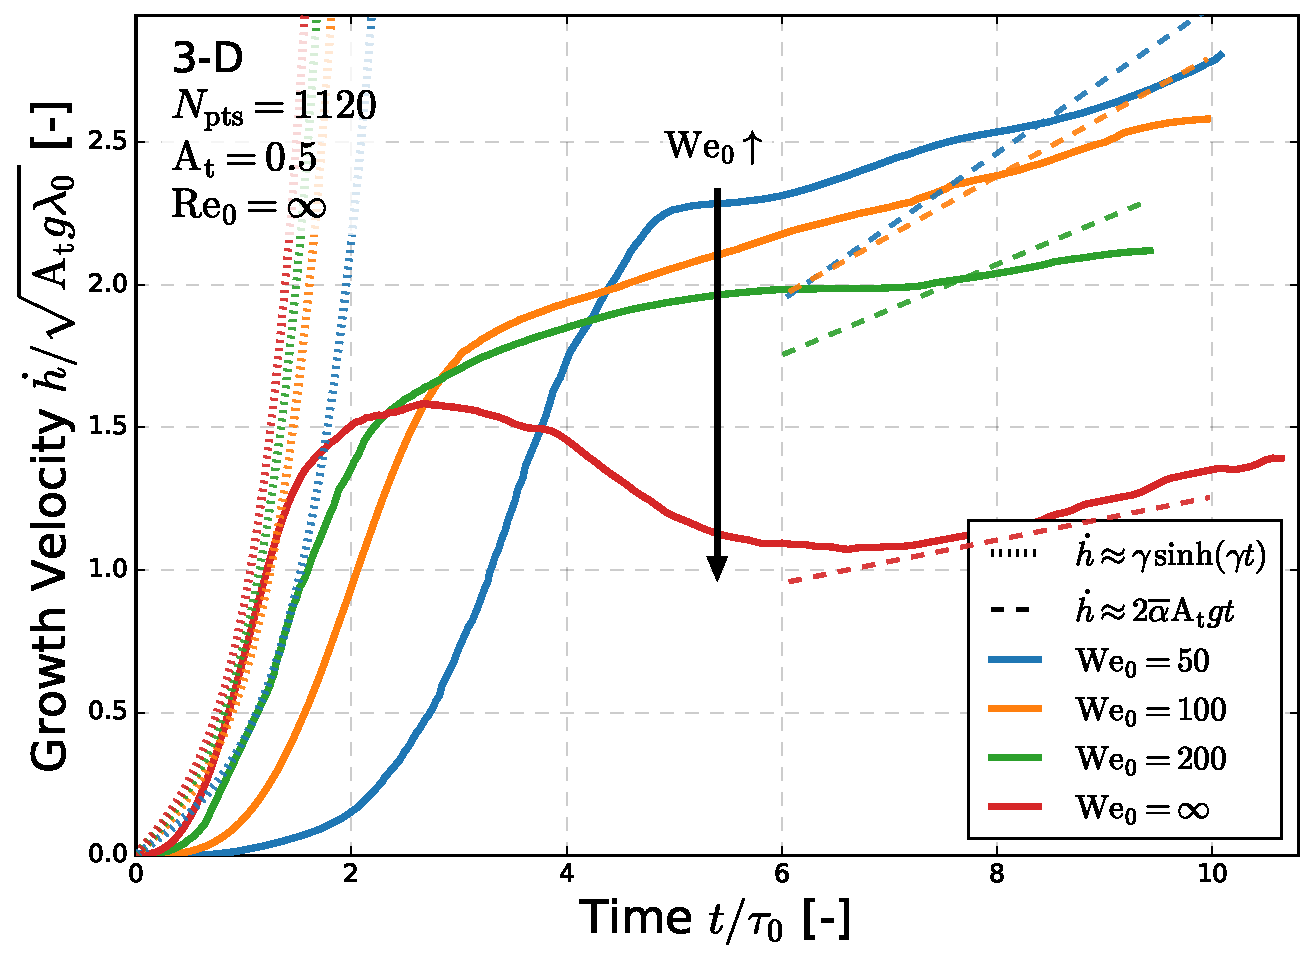
\includegraphics[width=\linewidth]{figures/simulations/immiscible_alpha_time_velocity.pdf}\caption{}\label{fig:imm:hdot}
\end{subfigure}
\caption{Immiscible simulations at $\We = 50$, $100$, $200$ and $\infty$, 3-D, $N_\mathrm{pts} = 1120$, $\At = 0.5$, $\mathrm{Re}_0 = \infty$ \cite{Walker2025,Walker2026}. Panels and line styles as in Figure~\ref{fig:misc}.}
\label{fig:imm}
\end{figure}

\subsection{Miscible and immiscible cases}\label{sec:sims:misc}
Figure~\ref{fig:misc} compares the miscible and immiscible cases without surface tension. The two follow the same linear and early nonlinear growth (Figures~\ref{fig:misc:h} and \ref{fig:misc:hdot}) and the same peak in $\alpha(t)$ near $t \approx 1.3 \tau_0$ (Figure~\ref{fig:misc:alpha}). After the transition, the immiscible layer grows faster, and $\alpha(t)$ settles at $\alpha_{\rm imm} \approx 0.039$ compared with $\alpha_{\rm misc} \approx 0.028$. In both cases, the late-time growth velocity increases approximately linearly in time (Figure~\ref{fig:misc:hdot}), as expected for quadratic growth.

\subsection{Transition}\label{sec:sims:transition}
Decreasing $\We$ delays the transition and lowers the peak of $\alpha(t)$ (Figure~\ref{fig:imm:alpha}). The time of maximum $\mathrm d \bar\theta/\mathrm d t$ marked in Figure~\ref{fig:imm:h}, $t_\theta$, and the time of peak $\alpha$, $t_{\rm peak}$, both increase linearly with $\We^{-1}$, that is linearly with $\sigma$ (Figure~\ref{fig:transition:time}):
\begin{equation}\label{eq:t_transition}
\frac{t_\theta}{\tau_0} \approx 1.88 + \frac{179}{\We} \, , \qquad \frac{t_{\rm peak}}{\tau_0} \approx 1.15 + \frac{139}{\We} \;,
\end{equation}
with root-mean-square deviations of $0.03$ and $0.13$ over the four cases, including $\We = \infty$. A delay linear in $\sigma$ is the form expected from the first-order capillary correction to the growth rate \eqref{eq:dispersion}. Aligned at $t_\theta$ (Figure~\ref{fig:transition:alpha}), the finite-$\We$ curves nearly coincide for $(t - t_\theta)/\tau_0 \lesssim 3$; the ratio of the largest to the smallest $\alpha$ among $\We = 50$--$200$ rises from $1.04$ at $(t - t_\theta)/\tau_0 = 2$ to $1.32$ at $4.5$, and the ratio to $\We = \infty$ from $1.3$ to $2.8$. Cook \& Dimotakis \cite{Cook2001} found that a progress variable brings cases with different initial conditions into closer agreement than time does, and RC04 attribute this to the virtual origin.

\begin{figure}[h!]
\centering
\begin{subfigure}[t]{0.478\textwidth}\centering
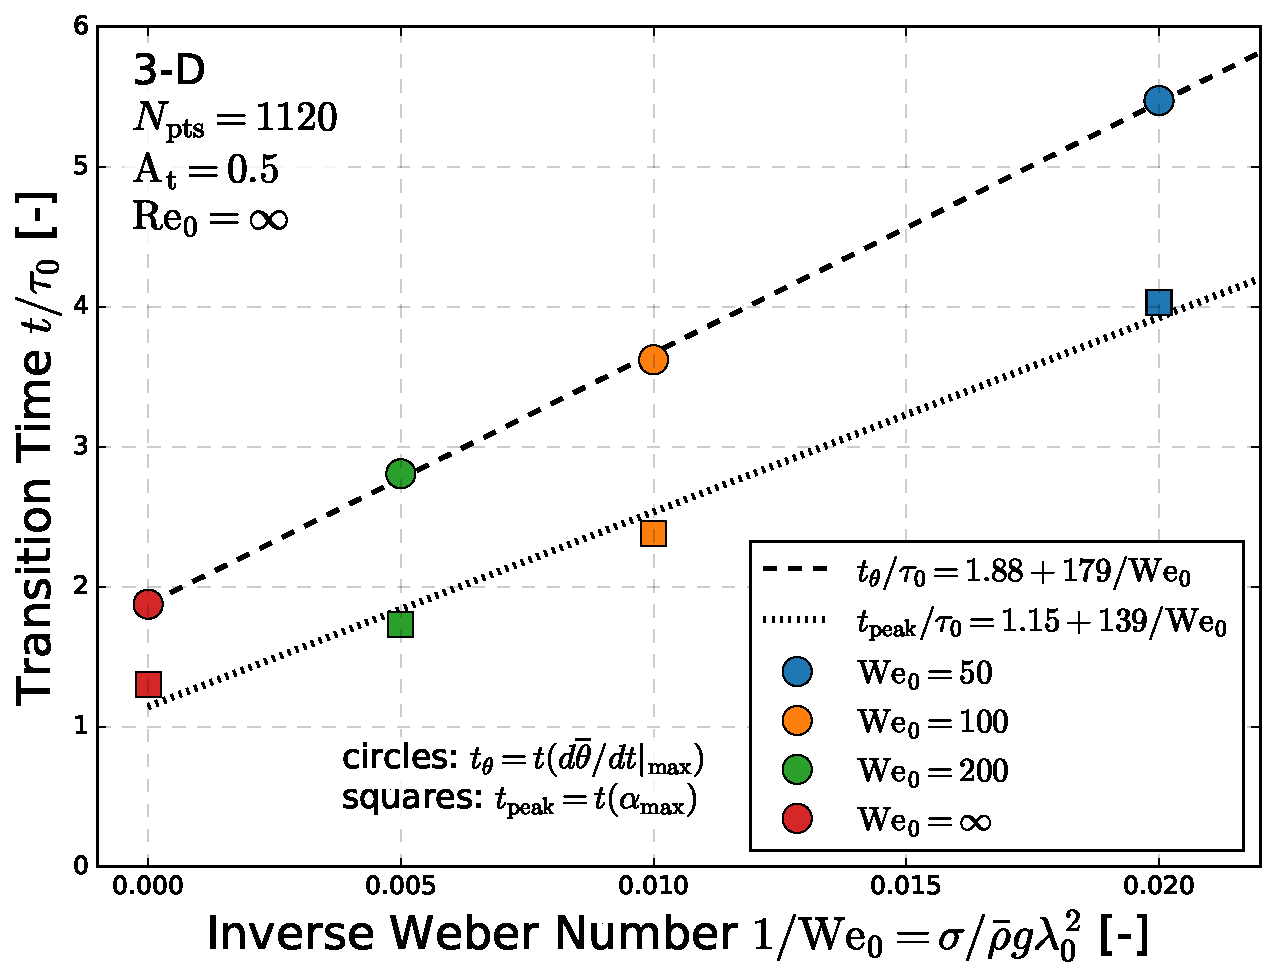
\includegraphics[width=\linewidth]{figures/fig_transition_time.pdf}\caption{}\label{fig:transition:time}
\end{subfigure}\hfill
\begin{subfigure}[t]{0.49\textwidth}\centering
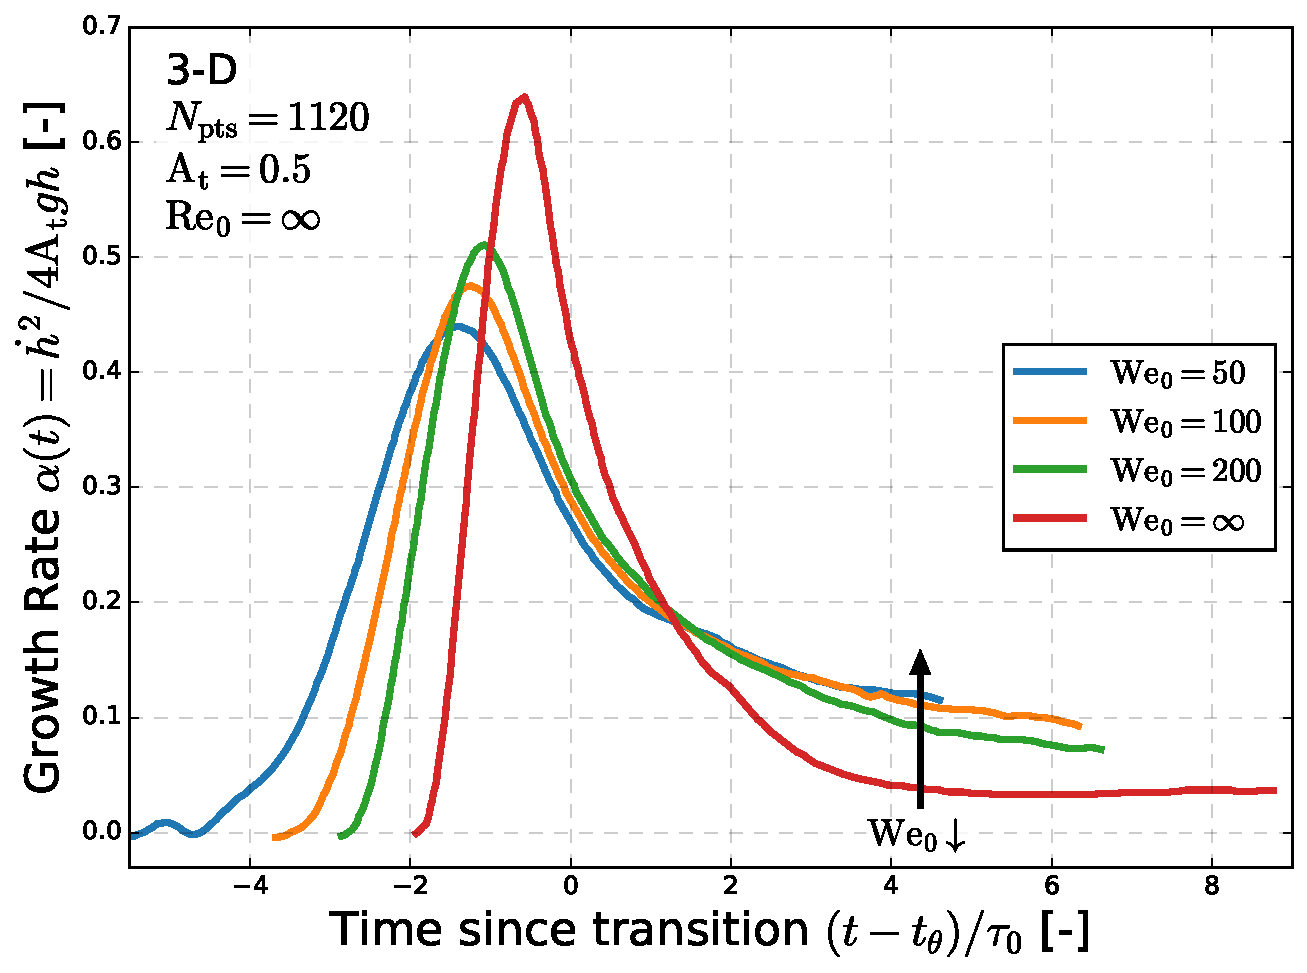
\includegraphics[width=\linewidth]{figures/fig_alpha_transition.pdf}\caption{}\label{fig:transition:alpha}
\end{subfigure}
\caption{(a) Transition time against $1/\We$: time of maximum $\mathrm d \bar\theta/\mathrm d t$ (circles) and of peak $\alpha$ (squares), with the fits \eqref{eq:t_transition}. (b) Growth parameter against time since $t_\theta$.}
\label{fig:transition}
\end{figure}

\subsection{Comparison at fixed time}\label{sec:sims:fixed}
Table~\ref{tab:fixed_time} lists the ratio $\alpha(\We {=} 50)/\alpha(\We {=} 200)$ at fixed $t/\tau_0$ and the corresponding effective power law. At $t \approx 10 \tau_0$, this is close to the fit $0.49 \, \We^{-0.35}$ of Ref.~\cite{Walker2026}. The form $\alpha \approx \alpha_\infty + K \We^{-1/2}$ also fits at any single time, with $\alpha_\infty \approx 0.030$--$0.035$, but $K$ drops from $1.2$ at $6 \tau_0$ to $0.62$ at $9.4 \tau_0$. The exponent obtained at fixed time is therefore not a property of the flow; it depends on when the simulations are compared.
\begin{table}[h!]
\centering
\caption{Growth parameter compared at fixed time, from the curves of Figure~\ref{fig:imm:alpha}.}
\label{tab:fixed_time}
\begin{tabular}{ccc}
\toprule
$t/\tau_0$ & $\alpha(\We {=} 50)/\alpha(\We {=} 200)$ & effective scaling\\
\midrule
6.0 & 1.89 & $\We^{-0.46}$\\
6.5 & 1.80 & $\We^{-0.43}$\\
7.5 & 1.84 & $\We^{-0.44}$\\
8.5 & 1.66 & $\We^{-0.37}$\\
9.4 & 1.68 & $\We^{-0.38}$\\
\bottomrule
\end{tabular}
\end{table}

\subsection{Comparison at equal mixing width}\label{sec:sims:width}
Figure~\ref{fig:excess:alpha} shows $\alpha$ against $h/\lambda_0$. Without surface tension, $\alpha$ settles at $0.034$--$0.036$ for $h/\lambda_0 \gtrsim 8$. With surface tension, it continues to decrease, as $\alpha \propto (h/\lambda_0)^{-0.6}$ to $(h/\lambda_0)^{-0.85}$, and remains two to five times larger at equal width. Over the range $7 \le h/\lambda_0 \le 12.5$, in which all four cases overlap, the excess $\alpha - \alpha_{\We = \infty}$ evaluated at equal $h$ collapses onto a single line when plotted against $\ls/h$ (Figure~\ref{fig:excess:fit}):
\begin{equation}\label{eq:excess_fit}
\alpha - \alpha_{\We = \infty} \approx 8.9 \, \frac{\ls}{h} \;,
\end{equation}
with the coefficient between $7.7$ and $9.9$ over all three Weber numbers and a fitted slope of $0.97$ on logarithmic axes. This is the form \eqref{eq:linear_We} with $K \approx 8.9$: at fixed $h/\lambda_0$ the excess is proportional to $\We^{-1/2}$, and at fixed $\We$ it decays as $h^{-1}$. Compared with the models of Section~\ref{sec:scaling}, the exponent agrees with the spectral closure for $D_s = 2$ and with the capillary-velocity form \eqref{eq:capvel}, while the magnitude is about $250$ times that of the spectral closure ($K = \alpha_\infty$) and four orders of magnitude larger than the direct capillary correction \eqref{eq:scaling_rc}, which has the opposite sign.

\begin{figure}[h!]
\centering
\begin{subfigure}[t]{0.49\textwidth}\centering
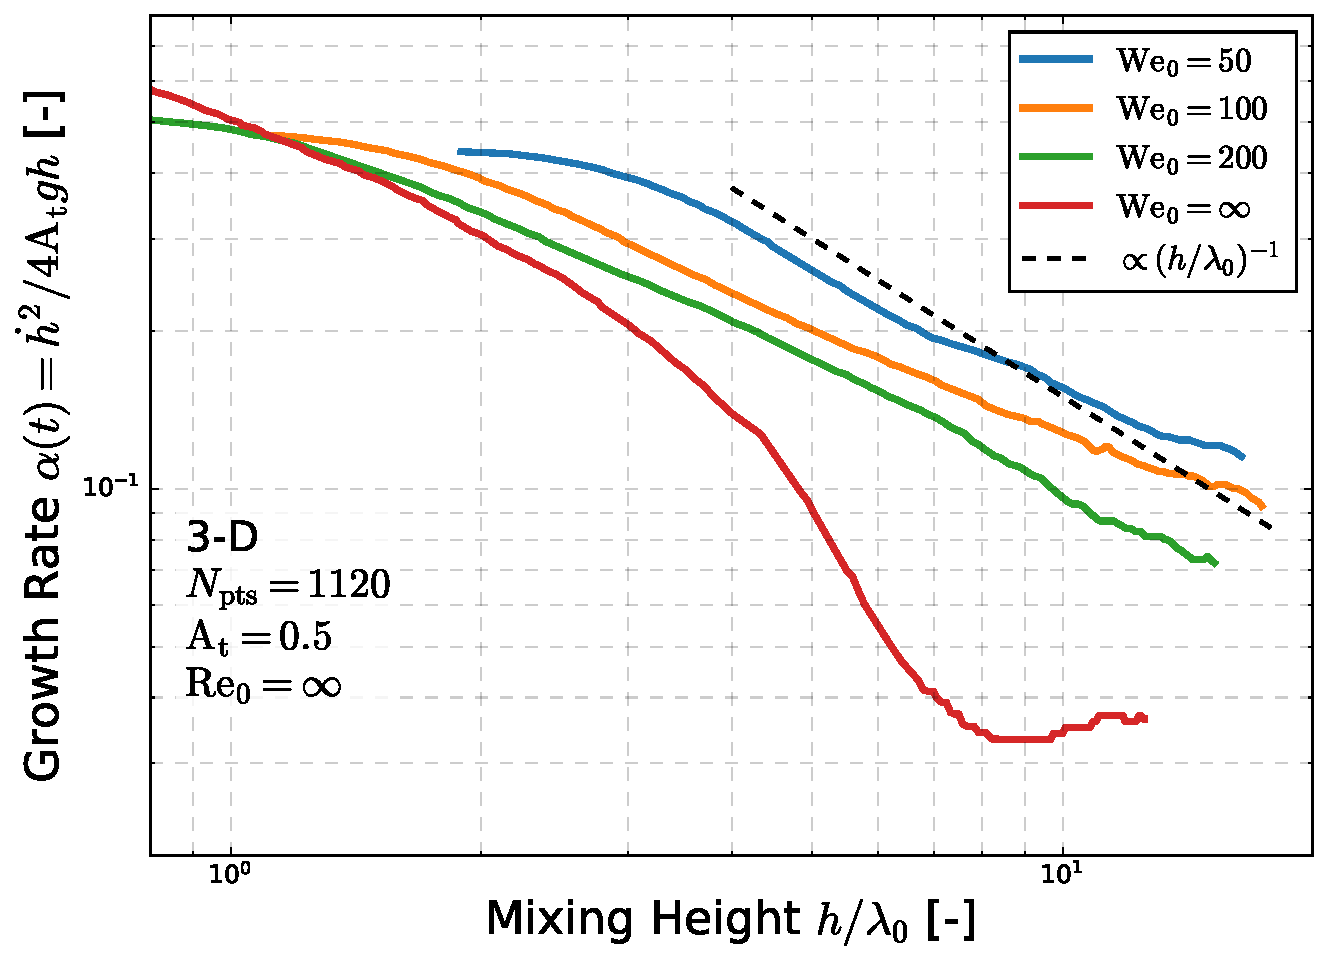
\includegraphics[width=\linewidth]{figures/fig_alpha_height.pdf}\caption{}\label{fig:excess:alpha}
\end{subfigure}\hfill
\begin{subfigure}[t]{0.49\textwidth}\centering
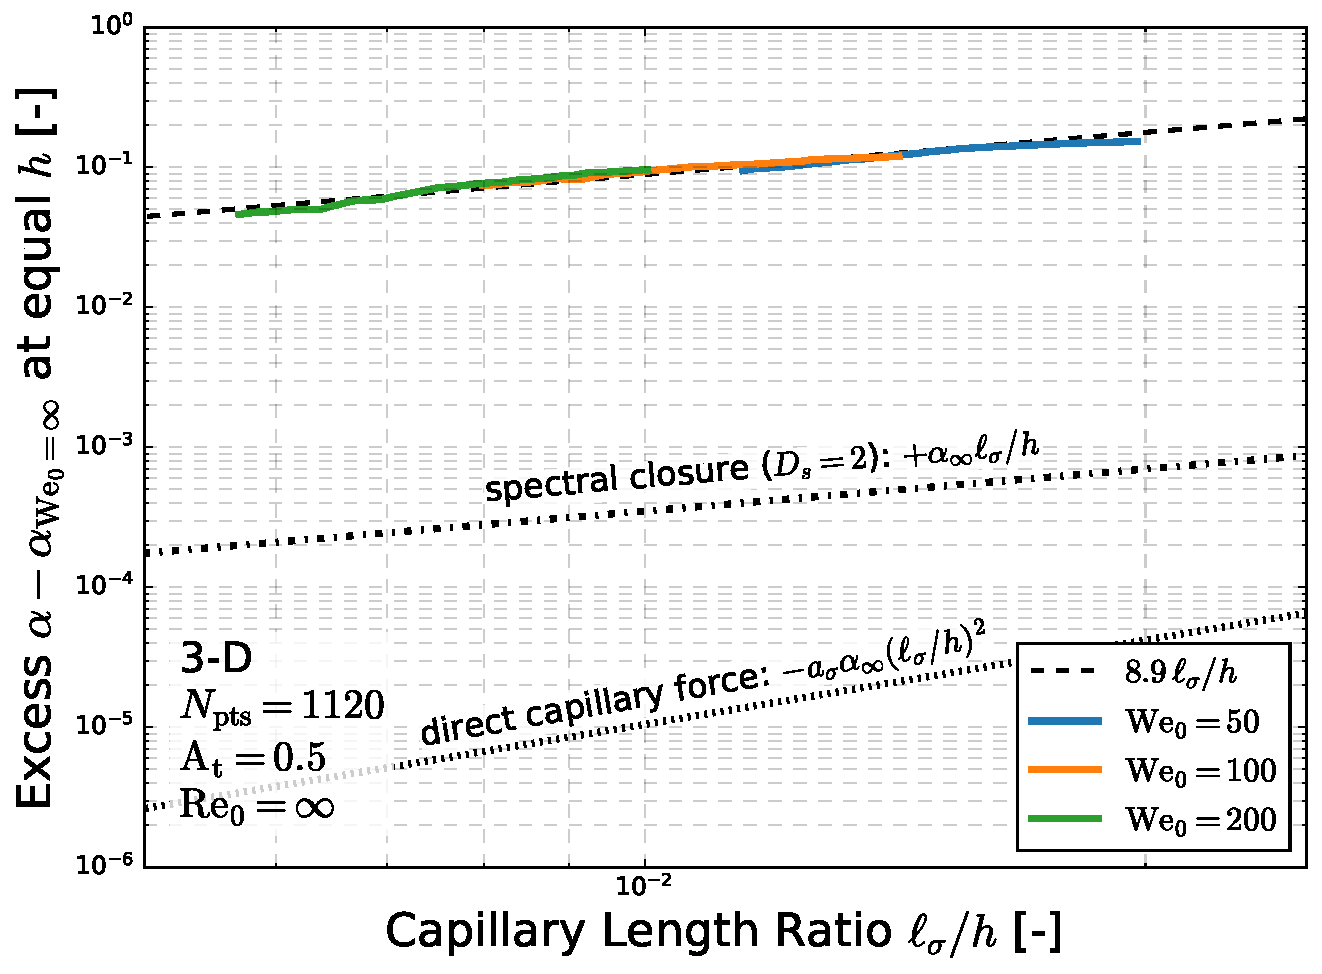
\includegraphics[width=\linewidth]{figures/fig_excess_width.pdf}\caption{}\label{fig:excess:fit}
\end{subfigure}
\caption{(a) Growth parameter against mixing height after the peak of $\alpha$. (b) Excess $\alpha - \alpha_{\We = \infty}$ at equal $h$ against $\ls/h$ for $7 \le h/\lambda_0 \le 12.5$, with the fit \eqref{eq:excess_fit}, the spectral closure \eqref{eq:alpha_closure} with $D_s = 2$, and the magnitude of the direct capillary correction \eqref{eq:alpha_t_corr} with $\nu = 2$ and $a_\sigma \approx 3$.}
\label{fig:excess}
\end{figure}

\subsection{Dependence on the comparison}\label{sec:sims:basis}
Figure~\ref{fig:exponent:m} shows the effective exponent $m$ in $\alpha \propto \We^{-m}$ across $\We = 50$--$200$ for three comparisons. At fixed $t/\tau_0$, $m$ decreases from $0.51$ to $0.38$ between $5.5 \tau_0$ and $9.4 \tau_0$, and the excess over $\We = \infty$ has $m \approx 0.55$--$0.68$. At fixed $h/\lambda_0$, $m$ for $\alpha$ is $0.25$--$0.37$, and for the excess it rises from $0.33$ to about $0.5$ as the $\We = \infty$ case settles. At fixed time since transition, $m$ rises from about zero to $0.2$. The exponent reported for a given set of simulations therefore depends on the basis of comparison. The comparison at equal width is the natural one for the analyses of Sections~\ref{sec:rc}--\ref{sec:scaling}, which are formulated in $h$.

Figure~\ref{fig:capgroup} shows the capillary group \eqref{eq:dsigma}, $1/\mathrm{We}(t)$. It falls below $10^{-2}$ after the transition and is $(1.5$--$3.2) \times 10^{-4}$ at the end of the simulations, so the direct capillary term in the flux budget is negligible at late times, in agreement with Section~\ref{sec:rc:capillary}.

\begin{figure}[h!]
\centering
\begin{subfigure}[t]{0.49\textwidth}\centering
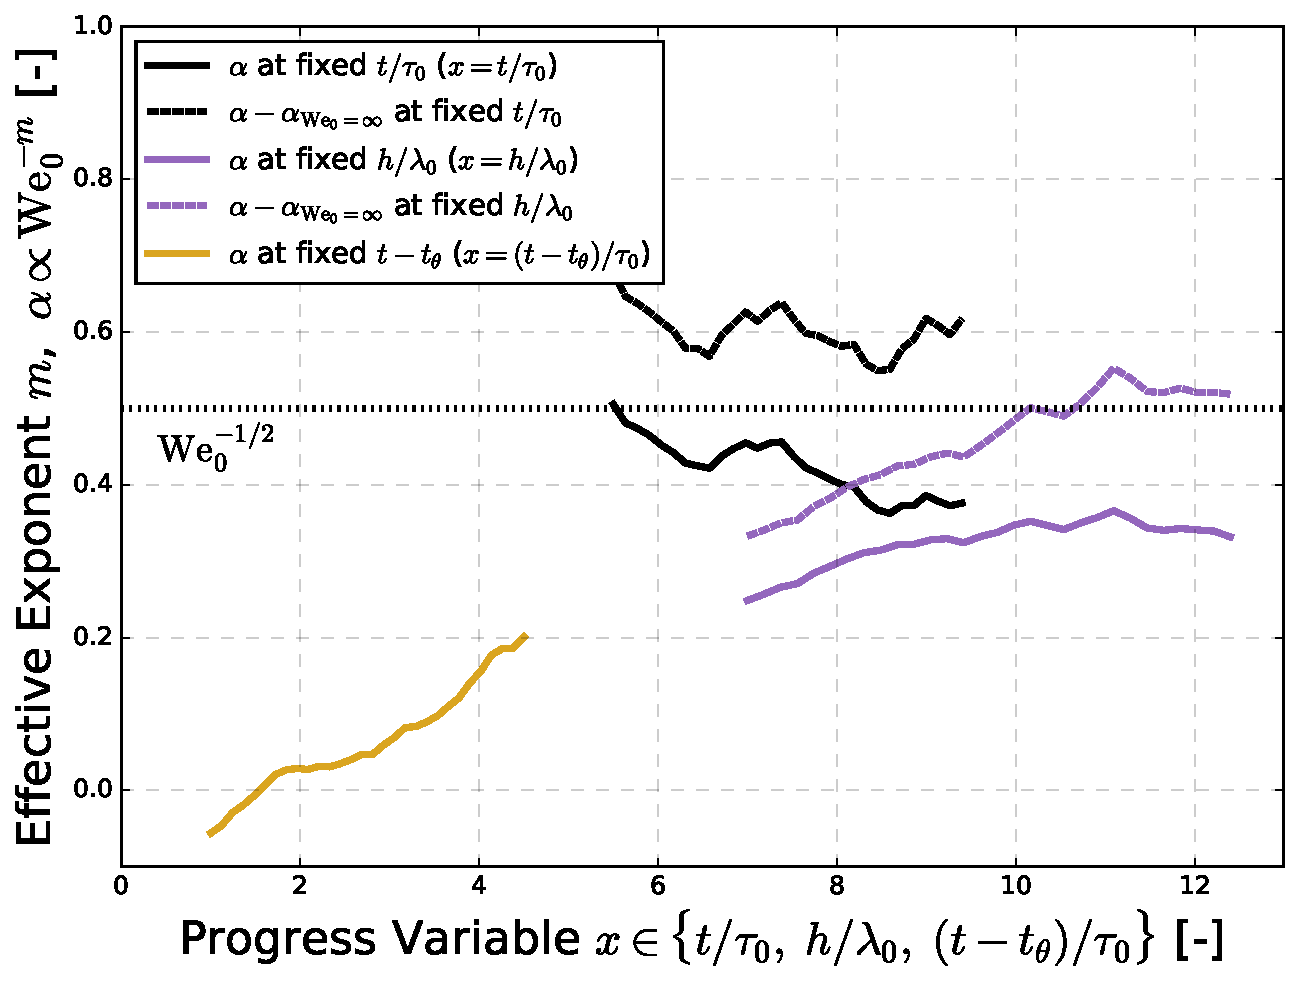
\includegraphics[width=\linewidth]{figures/fig_We_exponent.pdf}\caption{}\label{fig:exponent:m}
\end{subfigure}\hfill
\begin{subfigure}[t]{0.505\textwidth}\centering
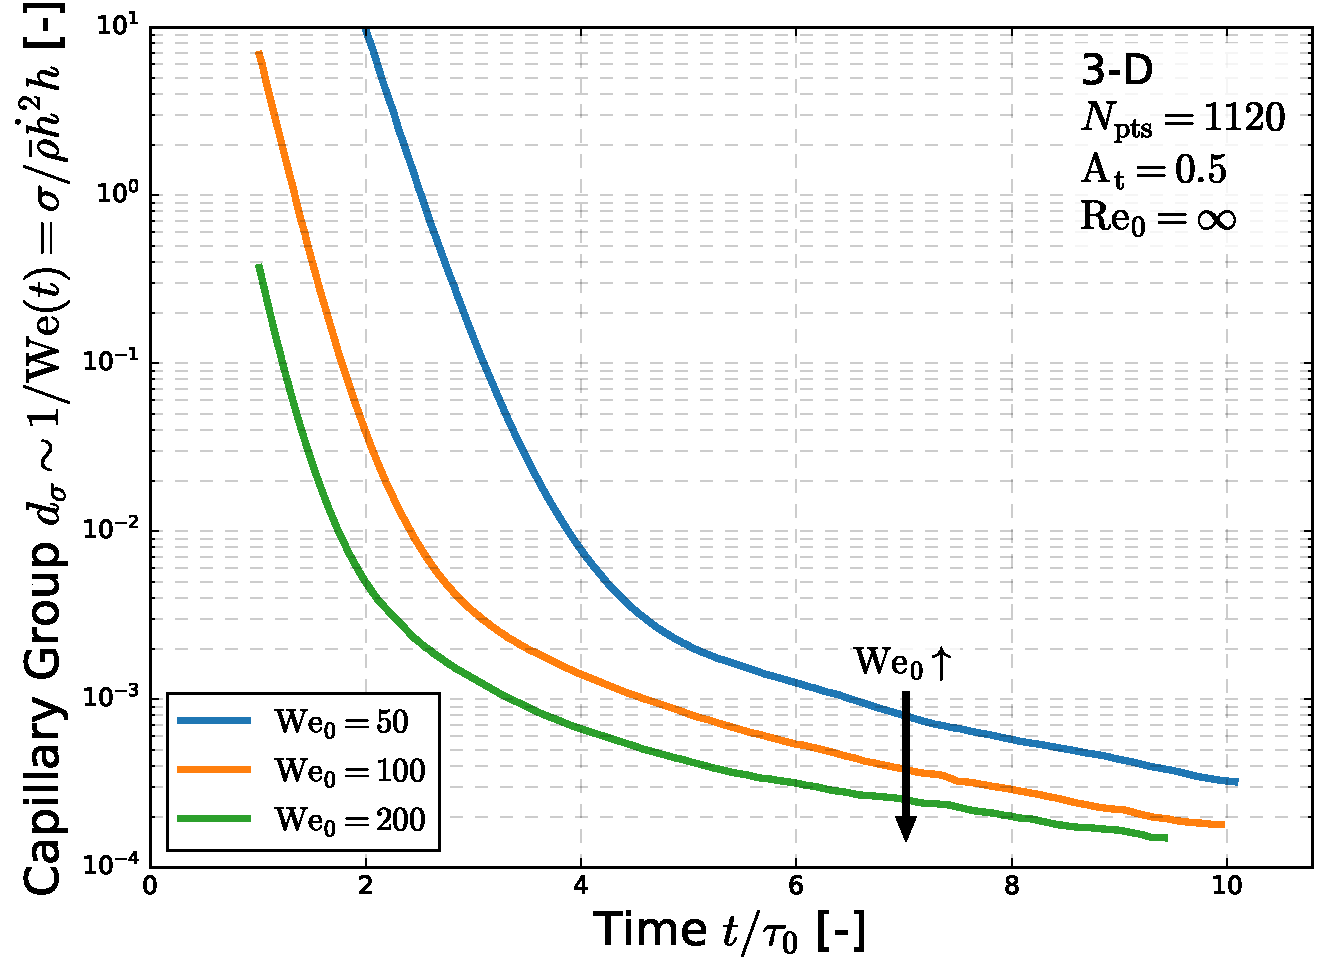
\includegraphics[width=\linewidth]{figures/fig_capillary_group.pdf}\caption{}\label{fig:capgroup}
\end{subfigure}
\caption{(a) Effective exponent $m$ in $\alpha \propto \We^{-m}$, fitted over $\We = 50$, $100$, $200$, for $\alpha$ and for $\alpha - \alpha_{\We = \infty}$ at fixed $t/\tau_0$ and at fixed $h/\lambda_0$, and for $\alpha$ at fixed $t - t_\theta$; the horizontal axis is the corresponding progress variable, $x = t/\tau_0$, $h/\lambda_0$ or $(t - t_\theta)/\tau_0$. (b) Capillary group $d_\sigma \sim 1/\mathrm{We}(t)$ \eqref{eq:dsigma}.}
\label{fig:exponent}
\end{figure}

\subsection{Resolution of the capillary scale}\label{sec:sims:resolution}
The capillary length is close to the grid spacing in these simulations. Taking $\lambda_0 = L/k_{\max} \approx 1.02$\,cm and $\Delta x = L/N_\mathrm{pts} \approx 0.114$\,cm, $\ls/\Delta x = 1.26$, $0.89$ and $0.63$ for $\We = 50$, $100$ and $200$, and the capillary cutoff wavelength $\ls$ spans $4$--$8 \, [\Delta x]$. That the excess is a single function of $\ls/h$ \eqref{eq:excess_fit} indicates that, over the simulated range, the late-time effect of surface tension is organized by $\ls$ even though $\ls$ is comparable to the grid spacing. The limit of drop breakup at the grid scale in these simulations is analyzed with a geometric model in Ref.~\cite{Walker2027_2}.

%======================================================================
\section{Summary}\label{sec:summary}
\begin{enumerate}
\item Dimensional analysis gives $\alpha = \Psi(t/\tau_0; \At, \We, \mathrm{Re}_0, \dots)$ \eqref{eq:pi} and does not fix the $\We$ dependence. A $\We^{-1/2}$ dependence is consistent with dimensional analysis as a correction $\alpha - \alpha_\infty = K \ls/h$ \eqref{eq:capvel}, produced by a velocity scale $(\At g \ls)^{1/2}$; it is not consistent with $\alpha \propto \We^{-1/2}$, which would vanish as $\sigma \rightarrowtriangle 0$. The instantaneous Weber number satisfies $\mathrm{We}(t) \propto \We(t/\tau_0)^4$ and $(\ls/h)^2 = 2 \alpha/\mathrm{We}(t)$ \eqref{eq:We_t}--\eqref{eq:ls_Wet}.
\item For immiscible fluids, $\avg{c' c'} = 1 - C^2$ \eqref{eq:constraint}, so the mixedness vanishes and the RC04 constant becomes $C_\mathrm{o} = (1 - \chi_0)/\hat D$ \eqref{eq:C0}: a buoyancy-efficiency factor divided by a normalized drag, both mid-plane statistics of the scalar-flux budget.
\item Under complete self-similarity, the capillary group is $1/\mathrm{We}(t) = (\ls/h)^2/2 \alpha$ \eqref{eq:dsigma}, so $\alpha_\infty$ is independent of $\We$. The first-order correction \eqref{eq:cap_ode} has the form \eqref{eq:mod_ode} with $\nu = 2$ and $a > 0$, and gives $\alpha - \alpha_\infty \propto -\We^{-1}$ \eqref{eq:scaling_rc}. Departures from self-similar growth in the RC04 balance with fixed constants decay as $h^{-R_f \hat D}$, with $R_f \hat D \approx 40$ \eqref{eq:relax_sol}.
\item The modified growth equation \eqref{eq:mod_ode} relates $\nu$ to the interface fractal dimension through \eqref{eq:mod_nu}, which follows from the indicator relations \eqref{eq:pq_Ds} and a Hinze-scale estimate of the capillary term \eqref{eq:hinze_estimate}; its effective growth parameter \eqref{eq:mod_aeff} is \eqref{eq:alpha_eff_corr} with $\nu = 1/5$. With $a > 0$, both diagnostics decrease with $\sigma$, and $\nu > 0$ requires $D_s < 7/3$.
\item For the full width \eqref{eq:h}, the self-similar mass-flux ratio is $R_f = 8.0$--$8.7$ \eqref{eq:Rf_values}; the simulations give $8.0$ without surface tension and $9.7$--$10.7$ with it. The decomposition \eqref{eq:decomp} divides the increase of $\alpha$ with decreasing $\We$ among comparable factors from $R_f^2$, the purity and $C_r^2 \mathrm{Fr}_0^2$ (Table~\ref{tab:decomp}); the purity factor alone overpredicts the miscible--immiscible difference.
\item A spectral closure beyond RC04 gives an increase of $\alpha$ with $\sigma$, $\alpha - \alpha_\infty \propto \We^{-(3 - D_s)/2}$ or $\We^{-3(3 - D_s)/5}$ \eqref{eq:We_scaling}; $D_s = 2$ with $\ell_{\rm in} = \ls$ gives $\nu = 1$ and $\We^{-1/2}$.
\item In the simulations, the transition time is linear in $\sigma$ \eqref{eq:t_transition}. At fixed time, the effective exponent drifts between $0.37$ and $0.46$ (Table~\ref{tab:fixed_time}). At equal mixing width, the excess over $\We = \infty$ follows a single curve, $\alpha - \alpha_\infty \approx 8.9 \, \ls/h$ \eqref{eq:excess_fit}, which is a $\We^{-1/2}$ dependence at fixed $h/\lambda_0$ and corresponds to $\nu = 1$ and $a \approx -250$ in \eqref{eq:mod_ode}.
\end{enumerate}

%======================================================================
\appendix
\section{Integration of the modified growth equation}\label{app:integration}
Let $\xi = (\ls/h)^{\nu}$. From \eqref{eq:cap_ode}, to first order in $\xi$,
\begin{equation}\label{eq:A1}
\hd = (\At g C_\mathrm{o} h)^{1/2} \Big[1 - \frac{a_\sigma}{2} \xi\Big] \;.
\end{equation}
Then $t = \int \mathrm d h/\hd$ gives, for $\nu \ne 1/2$,
\begin{equation}\label{eq:A2}
t = 2 \Big(\frac{h}{\At g C_\mathrm{o}}\Big)^{1/2} \Big[1 + \frac{a_\sigma}{2(1 - 2 \nu)} \, \xi\Big] + t_v \;,
\end{equation}
with $t_v$ a constant of integration. Substituting \eqref{eq:A1} and \eqref{eq:A2} into $\alpha_{\rm eff} = \hd/(2 \At g t)$ and expanding,
\begin{equation}\label{eq:A3}
\alpha_{\rm eff} = \frac{C_\mathrm{o}}{4} \Big[1 - a_\sigma \Big(\frac12 + \frac{1}{2(1 - 2 \nu)}\Big) \xi - \frac{c_v}{\sqrt h}\Big]
= \frac{C_\mathrm{o}}{4} \Big[1 - a_\sigma \, \frac{1 - \nu}{1 - 2 \nu} \, \xi - \frac{c_v}{\sqrt h}\Big] \;,
\end{equation}
with $c_v = \tfrac12 t_v(\At g C_\mathrm{o})^{1/2}$, which is \eqref{eq:alpha_eff_corr}. Squaring \eqref{eq:A1} and dividing by $4 \At g h$ gives \eqref{eq:alpha_t_corr}.

%======================================================================
\section*{List of symbols}
\phantomsection\addcontentsline{toc}{section}{List of symbols}
Dimensions are given in terms of mass M, length L and time T; a dash marks a dimensionless quantity. The last column gives the equation, section, figure or table in which the symbol is defined or first used. A symbol with more than one meaning has one row per meaning.

\subsection*{Roman symbols}
\begin{longtable}{@{}P{0.13}P{0.53}P{0.13}P{0.13}@{}}
\toprule
Symbol & Description & Dimensions & Defined in\\
\midrule
\endhead
\bottomrule
\endfoot
$a$ & Coefficient of the correction in the modified growth equation; $a < 0$ is required for $\alpha$ to increase with $\sigma$ & -- & \eqref{eq:mod_ode}\\
$a_\sigma$ & Coefficient of the first-order capillary correction, $a_\sigma = \hat d_\sigma/\hat D > 0$; the value of $a$ in \eqref{eq:mod_ode} for $\nu = 2$ & -- & \eqref{eq:cap_ode}\\
$\At$ & Atwood number, $\Delta \rho/(2 \bar\rho) = (\rho_h - \rho_\ell)/(\rho_h + \rho_\ell)$; $0.5$ in the simulations & -- & \eqref{eq:params}\\
$\mathrm{A}_\mathrm{eff}$ & Effective Atwood number of CCM04, $\At(1 - \theta_0)^{1/2}$ & -- & \S\ref{sec:cook:decomp}\\
$c$ & Phase indicator, $+1$ in the heavy fluid and $-1$ in the light fluid, so that $\rho = \bar\rho(1 + \At c)$ & -- & \S\ref{sec:rc:eqs}\\
$c'$ & Fluctuation of the indicator about its plane average, $c' = c - C$ & -- & \S\ref{sec:rc:eqs}\\
$\hat c_{\mathbf k}$ & Fourier coefficient of $c'$ at wavevector $\mathbf k$ & -- & \S\ref{sec:rc:flux}\\
$c_K$ & Shape coefficient of the kinetic energy, $K_E = c_K \bar\rho \, \hd^2 h$ & -- & \eqref{eq:energy}\\
$c_P$ & Shape coefficient of the released potential energy, $P_{\rm rel} = c_P \, \Delta \rho \, g h^2$; $1/24$ for a linear $\bar V$ profile & -- & \eqref{eq:energy}\\
$c_v$ & Virtual-origin coefficient in $\alpha_{\rm eff}$, $c_v = \tfrac12 t_v(\At g C_\mathrm{o})^{1/2}$ & L$^{1/2}$ & \eqref{eq:alpha_eff_corr}, \eqref{eq:A3}\\
$C$ & Plane-averaged indicator, $C = \avg c = 2 \bar V - 1$; $C = 0$ on the mid-plane & -- & \S\ref{sec:rc:eqs}\\
$C_\mathrm{o}$ & Growth constant of RC04, $\hd^2 = \At g C_\mathrm{o} h$; the constant amplitude of the mean indicator in the self-similar form; $C_\mathrm{o} = 4 \alpha_\infty$ & -- & \eqref{eq:C0}\\
$C_H$ & Constant in the Hinze scale, $C_H \approx 0.725$ & -- & \eqref{eq:hinze}\\
$C_r$ & Correlation coefficient of the mid-plane mass flux, $\avg{\rho' w'}_0 = -C_r \rho_{\rm rms} w_{\rm rms}$ (CCM04 eq.~7.5) & -- & \S\ref{sec:cook:decomp}\\
$C_w$ & Constant in the CCM04 velocity closure, $w_{\rm rms} = C_w(\mathrm{A}_\mathrm{eff} g h)^{1/2}$ & -- & \eqref{eq:cook_closure}\\
$C_\varepsilon$ & Dissipation coefficient, $\varepsilon_0 = C_\varepsilon \hd^3/h$ & -- & \S\ref{sec:rc:capillary}\\
$d_\mu$ & Normalized mid-plane sink of $F$ from viscosity, $(h/\hd^2)(\mu/\bar\rho) \avg{c' \nabla^2 w}_0$ & -- & \eqref{eq:groups}\\
$d_N$ & Normalized mid-plane sink of $F$ from the nonlinear pressure $p_N$ & -- & \eqref{eq:groups}\\
$d_T$ & Normalized mid-plane sink of $F$ from turbulent transport, $\partial \avg{w w c'}/\partial z$ & -- & \eqref{eq:groups}\\
$d_\sigma$ & Capillary group: normalized mid-plane sink of $F$ from the solenoidal capillary force; $d_\sigma \sim 1/\mathrm{We}(t)$ & -- & \eqref{eq:groups}, \eqref{eq:dsigma}\\
$\hat d_\sigma$ & Amplitude of the capillary group, $d_\sigma = \hat d_\sigma(\ls/h)^{\nu}$ & -- & \eqref{eq:dsigma_power}\\
$\hat D$ & Normalized inertia and drag in the mid-plane flux budget, $\hat D = 1/R_f + d_T + d_N + d_\mu - \hat w \, f_C'(0)$ & -- & \eqref{eq:flux_ode}\\
$D_s$ & Fractal dimension of the interface; $2$ for a smooth interface and $7/3$ for an indicator with the Obukhov--Corrsin spectrum & -- & \eqref{eq:pq_Ds}\\
$\mathbf e_z$ & Upward unit vector & -- & \eqref{eq:mom}\\
$E$ & Constant of integration in the relaxation solution & L$^{2 + \beta}$T$^{-2}$ & \eqref{eq:relax_sol}\\
$E_c(k)$ & Wavenumber spectrum of the indicator, $E_c \propto k^{-p}$ & L & \S\ref{sec:modified:exponent}\\
$E_\varepsilon$ & Kinetic energy dissipated per unit horizontal area & M\,T$^{-2}$ & \eqref{eq:energy}\\
$\mathbf f$ & Capillary force per unit mass, $\mathbf f = \nabla \cdot \mathbf T^\sigma = (\sigma/\bar\rho) \, \kappa \, \hat{\mathbf n} \, \delta_s$; $f_z$ is its vertical component & L\,T$^{-2}$ & \S\ref{sec:rc:eqs}\\
$f(\eta)$ & Similarity profile of a self-similar quantity, $F(z, t) = F_\mathrm{o}(t) \, f(\eta)$ & -- & \S\ref{sec:rc:constraint}\\
$f_C(\eta)$ & Similarity profile of the mean indicator, $C = f_C(\eta)$; $f_C'(0) = h \, \partial C/\partial z |_0$ & -- & \S\ref{sec:rc:mean}\\
$F$ & (i) Mid-plane indicator flux, $F = -\avg{w c'}_0 = 2 \hd/R_f$ & L\,T$^{-1}$ & \S\ref{sec:rc:flux}\\
 & (ii) Generic self-similar quantity, $F(z, t) = F_\mathrm{o}(t) \, f(\eta)$, with temporal amplitude $F_\mathrm{o}(t)$ & varies & \S\ref{sec:rc:constraint}\\
$F_L$ & Fraction of the indicator variance in the energy-containing range $1/h \le k \le 2/h$ & -- & \eqref{eq:FL}\\
$\mathrm{Fr}_0$ & Mid-plane Froude number, $\mathrm{Fr}_0^2 = w_{\rm rms}^2/(\At g h)$ & -- & \S\ref{sec:cook:decomp}\\
$g$ & Gravitational acceleration, acting in the $-z$ direction & L\,T$^{-2}$ & \S\ref{sec:setup:params}\\
$h$ & Full mixing width, $h = 6 \int \bar V(1 - \bar V) \, \mathrm d z$; the total width of a linear profile & L & \eqref{eq:h}\\
$\hd$, $\ddot h$ & Growth velocity and acceleration of the mixing width & L\,T$^{-1}$, L\,T$^{-2}$ & \eqref{eq:alpha_defs}\\
$h_0$ & Width at $t = 0$ in the RC04 solution; offset of the quadratic fit in Figures~\ref{fig:misc} and \ref{fig:imm} & L & \eqref{eq:rc_solution}\\
$h_C$, $\hd_C$ & Entrainment length of CCM04, $h_C = 4 \int_{-\infty}^0 \bar V \, \mathrm d z$, and its growth velocity & L, L\,T$^{-1}$ & \S\ref{sec:cook:flux}, \eqref{eq:Rf_values}\\
$\mathbf I$ & Identity tensor & -- & \eqref{eq:Tsigma}\\
$k$, $\mathbf k$ & Wavenumber and wavevector; in \eqref{eq:dispersion} $k = 2 \pi/\text{wavelength}$; $k_z$ is the vertical component of $\mathbf k$ & L$^{-1}$ & \eqref{eq:dispersion}\\
$k_{\min}$, $k_{\max}$ & Smallest and largest mode numbers of the initial perturbation in a domain of width $L$; $\lambda_0 = L/k_{\max}$ & -- & \eqref{eq:We0}\\
$K$ & (i) Coefficient of the correction linear in $\ls/h$, $\alpha - \alpha_\infty = K \ls/h$; $K \approx 8.9$ in the simulations & -- & \eqref{eq:capvel}, \eqref{eq:excess_fit}\\
 & (ii) Coefficient of the fixed-time fit $\alpha \approx \alpha_\infty + K \We^{-1/2}$ & -- & \S\ref{sec:sims:fixed}\\
$K_E$ & Kinetic energy per unit horizontal area, $K_E = c_K \bar\rho \, \hd^2 h$ & M\,T$^{-2}$ & \eqref{eq:energy}\\
$K_H$ & Prefactor of the Hinze scale, $K_H = C_H \, C_\varepsilon^{-2/5}(2 \alpha)^{-3/5} \approx 3.3$ & -- & \eqref{eq:hinze_scaling}\\
$\ell_H$ & Hinze scale: the smallest interface scale that turbulence can deform & L & \eqref{eq:hinze}\\
$\ell_{\rm in}$ & Inner cutoff of the fractal range of the interface; the smaller of $\ls$ and $\ell_H$ & L & \S\ref{sec:scaling:closure}\\
$\ls$ & Capillary length, $(\sigma/\Delta \rho \, g)^{1/2}$; the inverse of the cutoff wavenumber of linear theory & L & \eqref{eq:dispersion}\\
$L$ & Width of the computational domain & L & \eqref{eq:We0}\\
$m$ & Effective exponent in $\alpha \propto \We^{-m}$ & -- & Fig.~\ref{fig:exponent}\\
$\hat{\mathbf n}$ & Unit normal to the interface, $\nabla c/| \nabla c |$ & -- & \eqref{eq:Tsigma}\\
$N_\mathrm{pts}$ & Number of grid points in each direction, $1120$ & -- & Fig.~\ref{fig:misc}\\
$p$ & (i) Pressure divided by $\bar\rho$; $p'$ is its fluctuation, split into buoyancy, nonlinear and capillary parts $p_B$, $p_N$ and $p_\sigma$ & L$^2$T$^{-2}$ & \eqref{eq:mom}, \eqref{eq:poisson}\\
 & (ii) Spectral exponent of the indicator, $E_c \propto k^{-p}$; $p = 2 q + 1 = 4 - D_s$ & -- & \eqref{eq:pq_Ds}\\
$P_{\rm rel}$ & Potential energy released per unit horizontal area & M\,T$^{-2}$ & \eqref{eq:energy}\\
$q$ & Exponent of the second-order structure function, $\mathcal S_2 \propto r^{2 q}$; $q = (3 - D_s)/2$ & -- & \eqref{eq:pq_Ds}\\
$r$, $\mathbf r$ & Separation distance and separation vector & L & \S\ref{sec:modified:exponent}\\
$R_f$ & Mass-flux shape factor, $R_f = \Delta \rho \, \hd/| \avg{\rho' w'}_0 |$; $2/R_f = \int_{-\infty}^0 (1 + f_C) \, \mathrm d \eta$, so that $\avg{w c'}_0 = -2 \hd/R_f$; $8.0$--$8.7$ for self-similar profiles; twice the scaling ratio of Refs.~\cite{Walker2026,Walker2027_1} & -- & \eqref{eq:Rf}, \eqref{eq:flux_mean}\\
$\mathrm{Re}_0$ & Reynolds number of the initial perturbation; $\mathrm{Re}_0 = \infty$ (no physical viscosity) in the simulations & -- & \eqref{eq:pi}\\
$S(t)$ & Interface area per unit horizontal area & -- & \eqref{eq:energy}\\
$t$ & Time & T & --\\
$t_\theta$ & Transition time: the time of maximum $\mathrm d \bar\theta/\mathrm d t$ & T & \eqref{eq:t_transition}\\
$t_{\rm peak}$ & Time of the peak of $\alpha(t)$ & T & \eqref{eq:t_transition}\\
$t_v$ & Constant of integration (virtual origin) in $t(h)$ & T & \eqref{eq:A2}\\
$t_\sigma$ & Capillary time, $(\bar\rho \lambda_0^3/\sigma)^{1/2}$ & T & \eqref{eq:tsigma}\\
$\mathbf T^\sigma$ & Capillary stress tensor divided by $\bar\rho$ & L$^2$T$^{-2}$ & \eqref{eq:Tsigma}\\
$\mathbf u$ & Velocity, $\mathbf u = (u, v, w) = (u_1, u_2, u_3)$; $u_i$ in index notation; $u_3 = w$ in the notation of RC04 & L\,T$^{-1}$ & \eqref{eq:mom}\\
$U_\sigma$ & Velocity scale formed from capillarity and buoyancy, $(\At g \ls)^{1/2}$ & L\,T$^{-1}$ & \eqref{eq:capvel}\\
$V$ & Volume fraction of the heavy fluid; $\bar V(z, t)$ is its plane average and $\bar V_0$ the mid-plane value & -- & \eqref{eq:h}\\
$w$ & Vertical (upward) velocity component; $w_{\rm rms}$ is its root-mean-square value on the mid-plane & L\,T$^{-1}$ & \S\ref{sec:rc:eqs}\\
$\hat w$ & Normalized mid-plane variance of the vertical velocity, $\avg{w w}_0/\hd^2$ & -- & \eqref{eq:groups}\\
$\We$ & Initial Weber number, $\bar\rho \, g \, \lambda_0^2/\sigma$ & -- & \eqref{eq:We0}\\
$\mathrm{We}(t)$ & Instantaneous Weber number, $\bar\rho \, \hd^2 h/\sigma$ & -- & \eqref{eq:We_t}\\
$x$ & Progress variable in Figure~\ref{fig:exponent}: $t/\tau_0$, $h/\lambda_0$ or $(t - t_\theta)/\tau_0$ & -- & Fig.~\ref{fig:exponent}\\
$\mathbf x$, $x_i$ & Position vector and its components & L & \eqref{eq:poisson}\\
$\Delta x$ & Grid spacing, $L/N_\mathrm{pts}$ & L & \S\ref{sec:sims:resolution}\\
$y$ & Square of the growth velocity, $y = \hd^2$ & L$^2$T$^{-2}$ & \eqref{eq:relax_ode}\\
$Y$ & Mass fraction of the heavy fluid & -- & \S\ref{sec:setup:diag}\\
$z$ & Vertical coordinate, positive upward; $z = 0$ is the mid-plane & L & \S\ref{sec:setup:params}\\
\end{longtable}

\subsection*{Greek symbols}
\begin{longtable}{@{}P{0.13}P{0.53}P{0.13}P{0.13}@{}}
\toprule
Symbol & Description & Dimensions & Defined in\\
\midrule
\endhead
\bottomrule
\endfoot
$\alpha$ & Growth parameter in $h \approx \alpha \At g t^2$ & -- & \S\ref{sec:intro}\\
$\alpha(t)$ & Instantaneous growth parameter, $\hd^2/(4 \At g h)$; the measure used in the simulations & -- & \eqref{eq:alpha_defs}\\
$\alpha_{\rm eff}$ & Effective growth parameter of RC04, $\mathrm d h/\mathrm d(\At g t^2) = \hd/(2 \At g t)$ & -- & \eqref{eq:alpha_defs}\\
$\alpha_\infty$ & Self-similar limit of $\alpha$ as $h/\ls \rightarrowtriangle \infty$, $\alpha_\infty = C_\mathrm{o}/4$ & -- & \eqref{eq:C0}\\
$\alpha_{\rm imm}$, $\alpha_{\rm misc}$ & Late-time $\alpha$ of the immiscible ($\We = \infty$) and miscible simulations, $\approx 0.039$ and $0.028$ & -- & \S\ref{sec:intro}\\
$\alpha_{\We = \infty}$ & $\alpha(t)$ of the immiscible simulation without surface tension, taken at the same $h$ & -- & \eqref{eq:excess_fit}\\
$\bar\alpha$ & Growth parameter of the quadratic fit $h \approx \bar\alpha \At g t^2 + h_0$ & -- & Fig.~\ref{fig:misc}\\
$\beta$ & Exponent of the decay of departures from $\hd^2 \propto h$, $\beta = R_f \hat D - 1$ & -- & \eqref{eq:relax_ode}\\
$\gamma$ & Linear growth rate of a mode of wavenumber $k$ & T$^{-1}$ & \eqref{eq:dispersion}\\
$\Gamma$ & Capillary moment per unit $\sigma/\bar\rho$, $\avg{c' f_z} = (\sigma/\bar\rho) \Gamma$; $\Gamma_0$ is its mid-plane value & L$^{-2}$ & \S\ref{sec:scaling:rc}\\
$\delta_s$ & Surface delta function, concentrated on the interface & L$^{-1}$ & \eqref{eq:Tsigma}\\
$\Delta \rho$ & Density difference, $\rho_h - \rho_\ell$ & M\,L$^{-3}$ & \eqref{eq:params}\\
$\varepsilon$ & Dissipation rate of turbulent kinetic energy per unit mass; $\varepsilon_0$ is its mid-plane value & L$^2$T$^{-3}$ & \eqref{eq:hinze}\\
$\eta$ & Similarity variable, $\eta = z/h$ & -- & \S\ref{sec:rc:mean}\\
$\theta$ & Mixedness; $\theta_0$ is its mid-plane value & -- & \S\ref{sec:rc:constraint}\\
$\bar\theta$ & Global mixedness of the layer, whose maximum rate of change defines $t_\theta$ & -- & Fig.~\ref{fig:misc}\\
$\theta_m$ & Molecular mixing parameter of RC04, $1 - \avg{c' c'}/[(1 - C)(1 + C)]$; zero for immiscible fluids & -- & \S\ref{sec:rc:constraint}\\
$\kappa$ & Curvature of the interface, $\kappa = -\nabla \cdot \hat{\mathbf n}$ & L$^{-1}$ & \S\ref{sec:rc:eqs}\\
$\lambda_0$ & Initial perturbation length: the wavelength of mode $k_{\max}$, $\lambda_0 = L/k_{\max}$ & L & \eqref{eq:We0}\\
$\mu$ & Dynamic viscosity; $\mu/\bar\rho$ is the kinematic viscosity & M\,L$^{-1}$T$^{-1}$ & \eqref{eq:mom}\\
$\nu$ & Exponent of the correction $(\ls/h)^{\nu}$; $2$ under complete self-similarity, $(7 - 3 D_s)/5$ from the Hinze-scale estimate and $\approx 1$ in the simulations & -- & \eqref{eq:dsigma_power}, \eqref{eq:mod_ode}\\
$\xi$ & Expansion variable, $\xi = (\ls/h)^{\nu}$ & -- & App.~\ref{app:integration}\\
$\rho$ & Density; $\avg\rho$ is its plane average and $\rho'$ its fluctuation & M\,L$^{-3}$ & \S\ref{sec:rc:eqs}\\
$\rho_h$, $\rho_\ell$ & Densities of the heavy and light fluids & M\,L$^{-3}$ & \S\ref{sec:setup:params}\\
$\bar\rho$ & Mean density, $\tfrac12(\rho_h + \rho_\ell)$ & M\,L$^{-3}$ & \eqref{eq:params}\\
$\rho_{\rm rms}$ & Root-mean-square density fluctuation on the mid-plane, $\Delta \rho \,[\bar V_0(1 - \bar V_0)(1 - \theta_0)]^{1/2}$ & M\,L$^{-3}$ & \S\ref{sec:cook:decomp}\\
$\sigma$ & Surface tension coefficient & M\,T$^{-2}$ & \S\ref{sec:setup:params}\\
$\Sigma$ & Surface density: interface area per unit volume; $\Sigma(r)$ is its value measured at resolution $r$ & L$^{-1}$ & \S\ref{sec:rc:capillary}\\
$\tau_0$ & Initial time scale, $(\lambda_0/\At g)^{1/2}$ & T & \eqref{eq:We0}\\
$\Phi$ & Dimensionless function giving $h/\lambda_0$ & -- & \eqref{eq:pi}\\
$\Phi_\varepsilon$ & Fraction of the released potential energy that is dissipated, $E_\varepsilon/P_{\rm rel}$ & -- & \eqref{eq:energy}\\
$\Phi_\sigma$ & Fraction of the released potential energy stored as surface energy, $\sigma(S - 1)/P_{\rm rel}$ & -- & \eqref{eq:energy}\\
$\chi$ & Fraction of the buoyancy production cancelled by the buoyancy pressure; $\chi_0$ is its mid-plane value; $0$ for vertical columns, $1/3$ for isotropic structures, $1$ for horizontal layers & -- & \eqref{eq:chi}\\
$\Psi$ & Dimensionless function giving $\alpha(t)$ & -- & \eqref{eq:pi}\\
\end{longtable}

\subsection*{Operators and calligraphic symbols}
\begin{longtable}{@{}P{0.13}P{0.66}P{0.13}@{}}
\toprule
Symbol & Description & Defined in\\
\midrule
\endhead
\bottomrule
\endfoot
$\avg{\cdot}$ & Average over a horizontal plane & \S\ref{sec:rc:eqs}\\
$(\cdot)'$ & Fluctuation about the plane average & \S\ref{sec:rc:eqs}\\
$\dot{(\cdot)}$, $\ddot{(\cdot)}$ & First and second time derivatives & \eqref{eq:alpha_defs}\\
$(\cdot) |_0$ & Evaluated on the mid-plane $z = 0$ & \eqref{eq:groups}\\
$\nabla^{-2}$ & Inverse Laplacian & \eqref{eq:chi}\\
$\mathcal{O}(\cdot)$ & Order of magnitude & \S\ref{sec:rc:capillary}\\
$\mathcal P$ & Projection onto the solenoidal (divergence-free) part, $\mathcal P \mathbf f = \mathbf f - \nabla p_\sigma$ & \S\ref{sec:rc:flux}\\
$\mathcal{S}_2(r)$ & Second-order structure function of the indicator, $\avg{[c(\mathbf x + \mathbf r) - c(\mathbf x)]^2}$ & \S\ref{sec:modified:exponent}\\
\end{longtable}

\subsection*{Subscripts and accents}
\begin{longtable}{@{}P{0.13}P{0.66}P{0.13}@{}}
\toprule
Symbol & Description & Defined in\\
\midrule
\endhead
\bottomrule
\endfoot
$(\cdot)_\mathrm{o}$ & Temporal amplitude in the RC04 self-similar form $F(z, t) = F_\mathrm{o}(t) \, f(\eta)$ & \S\ref{sec:rc:constraint}\\
$(\cdot)_0$ & On a statistic: value on the mid-plane $z = 0$. On $\lambda_0$, $\tau_0$, $\We$, $\mathrm{Re}_0$ and $h_0$: initial or reference value & \S\ref{sec:rc:constraint}\\
$(\cdot)_h$, $(\cdot)_\ell$ & Heavy and light fluid & \S\ref{sec:setup:params}\\
$(\cdot)_\infty$ & Self-similar limit $h/\ls \rightarrowtriangle \infty$; on $\We$, the case without surface tension & \eqref{eq:C0}\\
$(\cdot)_B$, $(\cdot)_N$, $(\cdot)_\sigma$ & Buoyancy, nonlinear and capillary parts of the pressure & \S\ref{sec:rc:flux}\\
$(\cdot)_T$, $(\cdot)_\mu$ & Turbulent-transport and viscous terms of the flux budget & \eqref{eq:groups}\\
$(\cdot)_C$ & On $f_C$: mean indicator. On $h_C$: entrainment length of CCM04 & \S\ref{sec:rc:mean}\\
$(\cdot)_H$ & Hinze scale & \eqref{eq:hinze}\\
$(\cdot)_L$ & Large (energy-containing) scales & \eqref{eq:FL}\\
$(\cdot)_{\rm in}$ & Inner cutoff & \S\ref{sec:scaling:closure}\\
$(\cdot)_{\rm eff}$ & Effective & \eqref{eq:alpha_defs}\\
$(\cdot)_{\rm imm}$, $(\cdot)_{\rm misc}$ & Immiscible and miscible simulations & \S\ref{sec:intro}\\
$(\cdot)_{\rm peak}$ & At the peak of $\alpha(t)$ & \eqref{eq:t_transition}\\
$(\cdot)_{\rm rel}$ & Released & \eqref{eq:energy}\\
$(\cdot)_{\rm rms}$ & Root mean square & \S\ref{sec:cook:decomp}\\
$(\cdot)_s$ & Surface ($\delta_s$, $D_s$) & \eqref{eq:Tsigma}\\
$(\cdot)_v$ & Virtual origin & \eqref{eq:A2}\\
$(\cdot)_z$ & Vertical component & \S\ref{sec:rc:eqs}\\
$(\cdot)_\theta$ & Defined by the mixedness & \eqref{eq:t_transition}\\
$\bar{(\cdot)}$ & On $V$: plane average. On $\theta$: global value. On $\rho$: mean of the two densities. On $\alpha$: fitted value & \eqref{eq:h}\\
$\hat{(\cdot)}$ & Normalized quantity ($\hat D$, $\hat d_\sigma$, $\hat w$), unit vector ($\hat{\mathbf n}$) or Fourier coefficient ($\hat c_{\mathbf k}$) & \eqref{eq:groups}\\
\end{longtable}

% \subsection*{Abbreviations}
% \begin{longtable}{@{}P{0.16}P{0.76}@{}}
% \toprule
% Abbreviation & Meaning\\
% \midrule
% \endhead
% \bottomrule
% \endfoot
% 3-D & Three-dimensional\\
% AFLES & Artificial-fluid large-eddy simulation \cite{Cook2007}\\
% CCM04 & Cook, Cabot \& Miller \cite{Cook2004}\\
% RC04 & Ristorcelli \& Clark \cite{Ristorcelli2004}\\
% RT & Rayleigh--Taylor\\
% \end{longtable}

\bibliographystyle{plain}
\bibliography{citations}

\end{document}